\documentclass[a4paper, 10pt]{article}

%\usepackage{cmap}
\usepackage[T2A]{fontenc}
\usepackage[utf8]{inputenc}
\usepackage[english, russian]{babel}
\usepackage{graphicx}
\usepackage[top=2cm, bottom=2cm, left=3cm, right=2cm]{geometry}
\graphicspath{./}
\usepackage{biblatex}
\addbibresource{lib.bib}
\linespread{1.5}
{\usefont{T2A}{Tempora-TLF}{m}{n}
\usepackage{amsmath}

\usepackage{ragged2e}
\justifying

\usepackage{listings}
\usepackage{color}


\begin{document}
	
\begin{titlepage}
	\fontsize{12pt}{12pt}\selectfont
	\begin{figure}[t!]
		\centering
		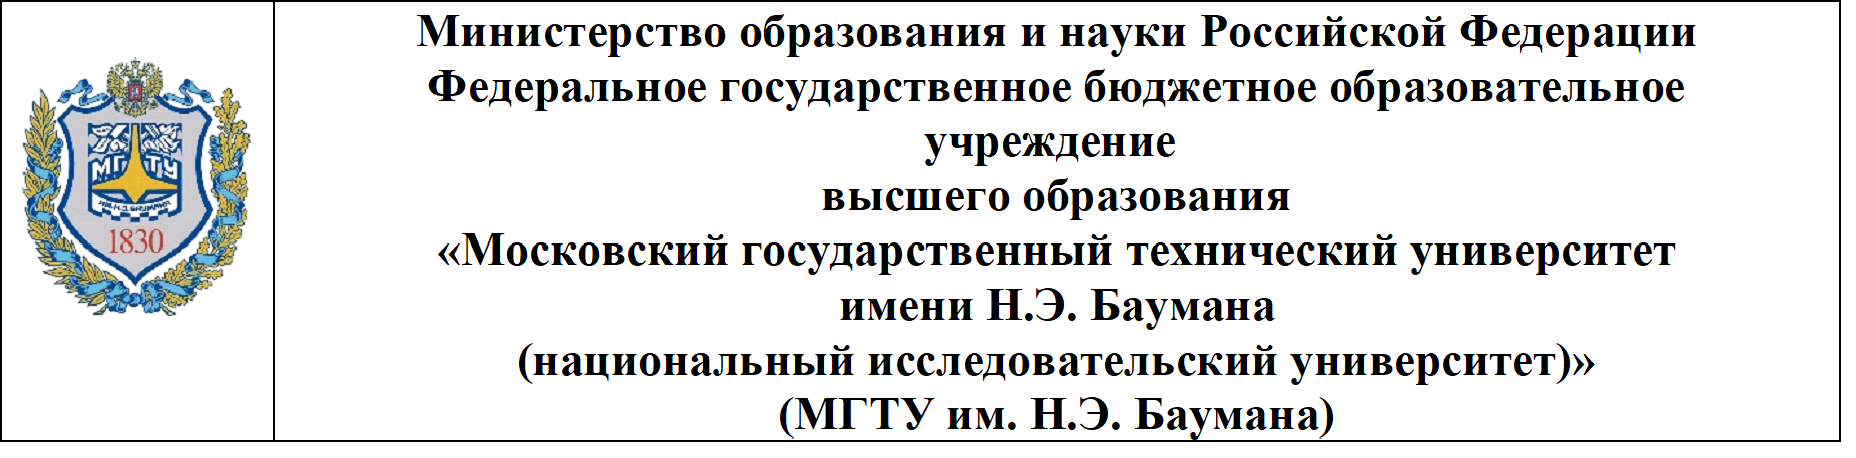
\includegraphics[scale=0.8]{bmstu}
	\end{figure}
	
	\noindent\rule{15cm}{3pt}
	\newline\newline
	\noindent 
	ФАКУЛЬТЕТ 
	\underline{«Информатика и системы управления»} \newline
	
	\noindent КАФЕДРА \underline{«Программное обеспечение ЭВМ и информационные технологии»}\newline\newline\newline\newline\newline
	
	\centering {\Large \textbf{\hspace*{1cm}РАСЧЕТНО-ПОЯСНИТЕЛЬНАЯ ЗАПИСКА}} 
	\newline \\ \centering{\Large \textbf{\textit{\hspace*{20mm}К КУРСОВОМУ ПРОЕКТУ}}}
	\newline \\ \centering{\Large \textbf{\textit{НА ТЕМУ:}}}
	\vspace{3mm}
	
	\centering{\LARGE \textrm{<<Генерация поверхностей трехмерного ландшафта>>}
		\vspace{10mm}	
		
	\vspace{10mm}}

	\begin{flushleft}
		Руководитель курсового проекта
		\hspace{2cm}$\underset{\text{(Подипсь, дата)}}{\underline{\hspace{4cm}}}$ 
		\hspace{4mm}$\underset{\text{(И.О.Фамилия)}}{\underline{\text{О.В.Кузнецова}}}$ 
	\end{flushleft}
    \begin{flushleft}
    	Студент
    	$\underset{\text{  (Группа)}}{\hspace{0.6cm}\underline{\hspace{0.6cm}\text{ИУ7-56Б}\hspace{0.6cm}}}$
    	\hspace{30mm}$\underset{\text{(Подипсь, дата)}}{\underline{\hspace{4cm}}}$ 
    	\hspace{4mm}$\underset{\text{(И.О.Фамилия)}}{\underline{\text{Ж.Р.Турсунов}}}$ 
    \end{flushleft}
	
	\begin{center}
		\vfill
		Москва, \the\year
		~г.
	\end{center}
	\clearpage
	\newpage
	\begin{center}
		\centering{\hspace{10mm} \footnotesize \bf Министерство науки и высшего образования Российской Федерации
			Федеральное государственное бюджетное образовательное учреждение
			высшего образования \\ <<Московский государственный технический университет имени Н.Э.Баумана\\(национальный исследовательский университет)>>\\(МГТУ им. Н.Э.Баумана)} 
		\noindent\rule{\textwidth}{2pt}
	\end{center}
	\begin{flushright}
		\small{УТВЕРЖДАЮ \\
		Заведующий кафедрой$\underset{\text{(Индекс)}}{\underline{\text{ИУ7}}}$ 
		\\ \vspace{1mm} $\underset{}{\underline{\hspace{3cm}}}$ \hspace{2mm}$\underset{\text{(И.О.Фамилия)}}{\underline{\text{И.В.Рудаков}}}$
		\\ \vspace{1mm}<<$\underset{}{\underline{\hspace{0.7cm}}}$ >> $\underset{}{\underline{\hspace{3cm}}}$2020 г.} 
	\end{flushright}

	\begin{center}
		\small{\bf{З А Д А Н И Е
		\\ на выполнение курсового проекта}}
	\end{center}
	\begin{flushleft}
		\small{по дисциплене $\underset{}{\underline{\hspace{2cm} \text{Компьютеная графика} \hspace{6.8cm}}}$
		\\Студент группы \underline{\hspace{1cm} \text{ИУ7-56Б} \hspace{1cm}}
		\\Тема курсового проекта \underline{\text{\hspace{1cm} Генерация поверхностей трехмерного ландшафта\hspace{0.7cm}}}
		\\ Направленность КП (учебный, исследовательский, практический, производственный, др.)
		\\ \underline{\hspace{6cm} \text{производственный} \hspace{6cm}}
		\\ Источник тематики (кафедра, предприятие, НИР)\underline{\hspace{2cm} \text{кафедра
			} \hspace{2.1cm}}
		\\График выполнения проекта:  25\% к \underline{4} нед., 50\% к \underline{7} нед., 75\% к \underline{11} нед., 100\% к \underline{14} нед.}
	\end{flushleft}
	 \begin{enumerate}
			\item \small {{ \textbf{\textit{Техническое задание}}} \underline{ Разработать программу генерации случайных поверхностей ландшафта на} \\ \underline{основе карт высот. Генерация изображения карты высот должен быть на основе «Шума Перлина»} \\ \underline{или «Холмового алгоритма». Пользователю необходимо дать выбор генерации одного из этих} \\ \underline{методов. Расчет карты освещенности ландшафта должен происходить с использованием нескольких} \\ \underline{источников света на основе метода Фонга. Также необходимо разработать две программы,  программу}\\ \underline{«Редактор» для генерации карты высот, расчета карты освещенности с поддержкой множества}\\  \underline{настроек и программу «Просмотр» для визуализации трехмерного ландшафта в реальном времени,} \\ \underline{в окружении воды и неба, на основе карт и текстур, сгенерированных заранее в программе} \\ \underline{«Редактор». Дать возможность для навигации по заданному миру.}}
			\item \small {{\textbf{\textit{Оформление курсового проекта}}}
			\begin{itemize}
				\item \footnotesize Расчетно-пояснительная записка на 30-35 листах формата А4.\\
				Расчетно-пояснительная записка должна содержать постановку введение, аналитическую часть, конструкторскую часть, технологическую часть, экспериментально-исследовательский раздел, заключение, список литературы, приложения.
				\item \small Перечень графического (иллюстративного) материала (чертежи, плакаты, слайды и т.п.)   
				На защиту проекта должна быть представлена презентация, состоящая из 15-20 слайдов. На слайдах должны быть отражены: постановка задачи, использованные методы и алгоритмы, расчетные соотношения, структура комплекса программ, диаграмма классов, интерфейс, характеристики разработанного ПО, результаты проведенных исследований.
		\end{itemize}}
		\end{enumerate}
		
		
		\begin{flushleft}
			\small Дата выдачи задания <<\underline{\hspace{1cm}}>> \underline{\hspace{3cm}} 2020 г.
			\\ \small \textbf{Руководитель курсового проекта}
			\small \hspace{3.45cm}$\underset{\text{(Подипсь, дата)}}{\underline{\hspace{4cm}}}$ 
			\small \hspace{4mm}$\underset{\text{(И.О.Фамилия)}}{\underline{\text{О.В.Кузнецова}}}$ 
		\end{flushleft}
		\begin{flushleft}
			\small \textbf{Студент}
			\small \hspace{7.7cm}$\underset{\text{(Подипсь, дата)}}{\underline{\hspace{4cm}}}$ 
			\small \hspace{4mm}$\underset{\text{(И.О.Фамилия)}}{\underline{\text{Ж.Р.Турсунов}}}$ 
		\end{flushleft}
	
\end{titlepage}
\setcounter{page}{3}
\tableofcontents
\clearpage
\newpage


\section*{Введение}
\addcontentsline{toc}{section}{Введение}

%\begin{flushleft}
	\hspace*{5mm}Роль компьютеров с каждым днём становится всё больше и больше. С каждым разом увеличивается область применения этой технологии. Для каждой области применения необходимы свои собственные программы, для решения конкретных задач. Благодаря этому в настоящее время постоянно появляются новые предметы изучения и исследования. Это целая наука, занимающаяся построением реальных графических изображений посредством вычислительных действий. Компьютерная графика закрепила за собой много важных задач, среди которых присутствуют такие, как визуализация результатов, полученных при обработке данных, моделирование реальных процессов и объектов. Военная область – одна из тех, кто не только первыми опробовали компьютеры, но и послужили в формирование компьютерной графики как науки. Например, для обучения и подготовки к действиям в боевых условиях пилотов самолетов, танков или какой-нибудь другой бронетехники, было необходимым создание симуляторов реальных технических средств. Было гораздо безопасно и эффективно, в плане военного бюджета посадить человека за симулятор для получения первоначальных навыков, чем на реальный объект. А для создания симулятора требовалось получать реалистичные изображения различных объектов, например, местности, на которой ведутся учения, причем эти изображения должны быть получены в реальном времени, то есть так, чтобы в зависимости от действий обучаемого соответственно менялись и параметры системы, такие как положение на местности, погодные условия. Спустя время стало ясно, что такие системы можно использовать не только для обучения новичков, но и для планирования реальных боевых операций на любой территории, о которой есть определенные данные.
	\\ \hspace*{5mm}«Трехмерное моделирование», ветвь 3D-моделирования, которая занимается проектированием и созданием трехмерных реалистичных изображений всех видов поверхностей и ландшафтов. 
	В настоящее время 3D-моделирование является важнейшей областью компьютерной графики, так как построение трехмерного изображения, близкого к реальному, является достаточно сложной задачей. Но, благодаря получаемым знаниям каждый день, невообразимому быстрому росту производительности вычислительных систем, эта область активно развивается.
	\\ \hspace*{5mm}Для простоты область 3D-моделирования можно разделить на 2 подобласти. Одна из них – это генерация трехмерных изображений в реальном времени, а другая – генерация высоко реалистичных трехмерных изображений. Высоко реалистичные изображения требуют очень больших объемов вычислений и производительности от машин, в то время как в первой подобласти применяется система условных допущений, позволяющая применять более простые алгоритмы, и тем самым значительно уменьшить объем вычислений, что, правда, сказывается на качестве изображения. Как уже было сказано, алгоритмы 3D-моделирования делятся на две группы.
	\\ \hspace*{5mm}В первую входят такие алгоритмы, как алгоритм Робертса, алгоритм Варнока, алгоритм, использующий z-буфер, которые в свою очередь используют простейшие алгоритмы построения линий, треугольников, закрашивание замкнутых областей. То есть алгоритмы, изученные нами в ходе курса «Компьютерной графики». Также к этой группе можно отнести алгоритмы, выполняющие отсечение.
	 
	Целью данной работы является генерация случайного трехмерного ландшафта. 
	\\Для достижения поставленной цели необходимо решить следующие задачи:
	\begin{enumerate}
		\item формализовать решаемую задачу;
		\item рассмотреть и проанализировать существующие алгоритмы решения задачи, выбрать подходящий;
		\item изучить физические принципы и законы, по которым строится выбранный метод визуализации;
		\item выбрать наиболее подходящую реализацию выбранного алгоритма;
		\item разработать архитектуру и структуру программы;
		\item выбрать средства программной реализации;
		\item разработать программные модули.
	\end{enumerate}
	
%\end{flushleft}
\clearpage
\newpage
\section{Аналитическая часть}
%\begin{flushleft}
	\hspace*{5mm} В данной части будут рассмотрены алгоритмы генерации, визуализации ландшафта и окружающей среды. 
	\subsection{Обзор и анализ существующего по и обоснование необходимости разработки}
	\hspace*{5mm} На сегоднешний день существуют множество программ генерирующих 3D ландшафт.\cite{po} К более известным можно отнести следующие программы:
	\begin{enumerate}
		\item Bryce;
		\item Vue 5 Esprit;
		\item MojoWorld;
		\item World Builder;
		\item VistaPro.
	\end{enumerate}
	\subsubsection{Bryce}
	{\bf Bryce} — одно из лучших профессиональных решений для моделирования как фотореалистичных, так и фантастических ландшафтов, позволяющее создавать миры с планетами, океанами, островами, горами и пр. Пакет прекрасно подходит в случаях разработки пейзажей для трехмерных игр, для оригинальных изображений в сфере полиграфии или видео и активно используется профессиональными дизайнерами.
	\\Недостатки:
	\begin{itemize}
		\item большой объем данных;
		\item большие требования к аппаратным ресурсам.
	\end{itemize}
	Преимущества:
	\begin{itemize}
		\item особые пакеты с частями пейзажа;
		\item расширенная поддержка экспорта и импорта.
	\end{itemize}
	На Рисунке 1 показан внутренний интерфейс программы Bryce.
	\clearpage
	\newpage
	\begin{figure}[h!]
		\centering
		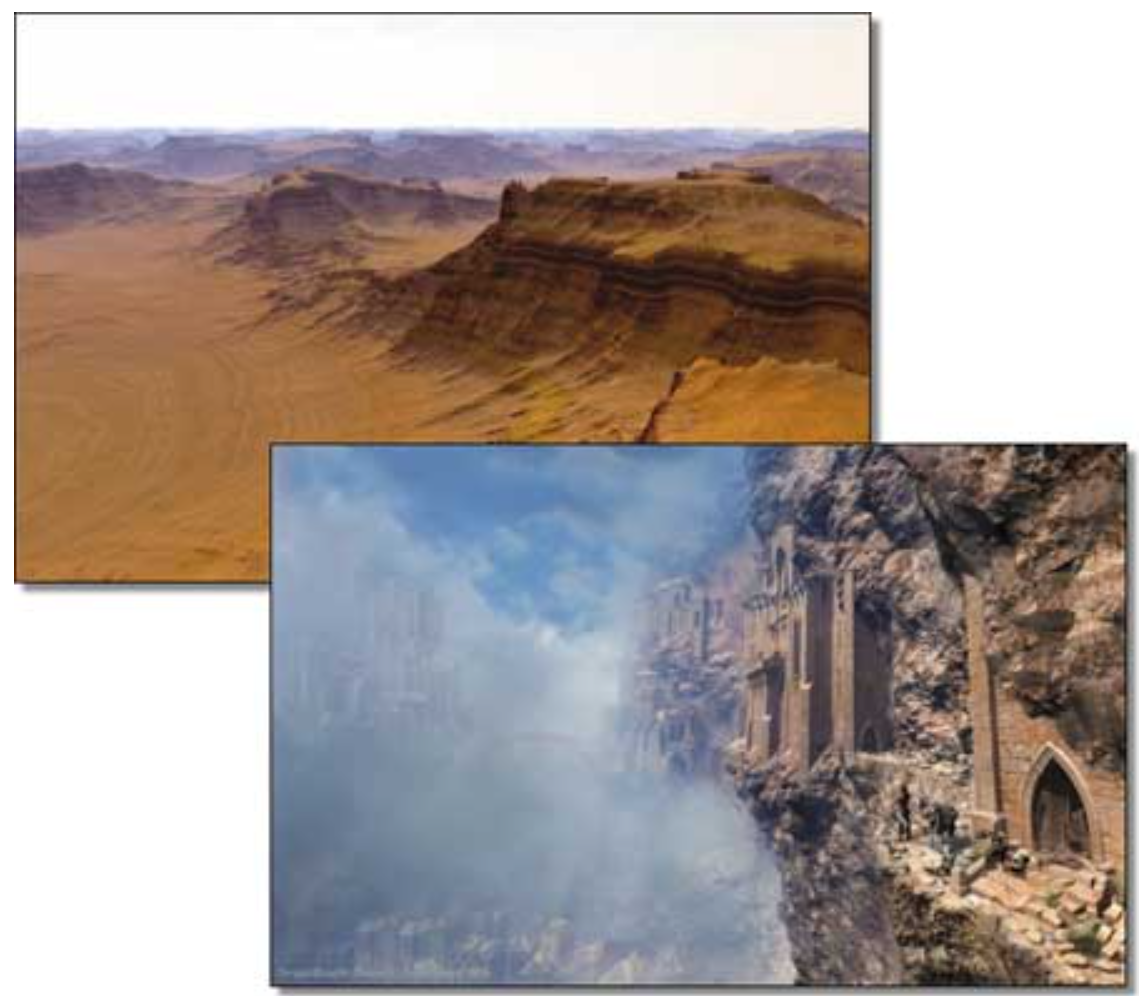
\includegraphics[scale=0.8]{bryce}
		\centering\caption{Интерфейс программы Bryce.}
	\end{figure}
	\subsubsection{Vue 5 Esprit}
 	{\bf Vue 5 Esprit} позволяет создавать как фотореалистичные, так и великолепные фантастические ландшафты с горами и водной гладью, великолепными атмосферными эффектами и разнообразной растительностью.
 		\\Недостатки:
 	\begin{itemize}
 		\item очень плохая поддержка импорта и экспорта;
 		\item слишком много ненужных возможностей.
 	\end{itemize}
 	Преимущества:
 	\begin{itemize}
 		\item более привычный интерфейс;
 		\item небольшой объем.
 	\end{itemize}
 	На Рисунке 2 показан внутренний интерфейс программы Vue 5 Esprit.
 	\clearpage
 	\newpage
 	\begin{figure}[h!]
 		\centering
 		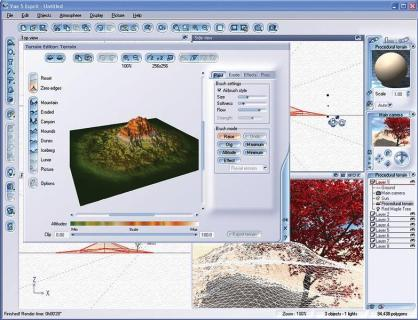
\includegraphics[scale=0.7]{vue}
 		\centering\caption{Интерфейс программы Vue 5 Esprit.}
 	\end{figure}
 	\subsubsection{VistaPro}
 	{\bf VistaPro} имеет самую длительную историю развития и когда-то работал еще под MS-DOS, позволяет строить как фотореалистичные пейзажи, полностью соответствующие существующим в действительности в том или ином уголке планеты, так и совершенно фантастические ландшафты, возникающие в воображении художника.
 	\\Недостатки:
 	\begin{itemize}
 		\item ограниченность баз данных объектов;
 		\item малое количество настроек для регулирования небесных, атмосферных и прочих ландшафтных параметров.
 	\end{itemize}
 	Преимущества:
 	\begin{itemize}
 		\item невысокие требования к аппаратным ресурсам;
 		\item поддержка баз данных ГИС;
 		\item небольшая цена.
 	\end{itemize}
 	На Рисунке 3 показан внутренний интерфейс программы VistaPro.
 	\clearpage
 	\newpage
 	\begin{figure}[h!]
 		\centering
 		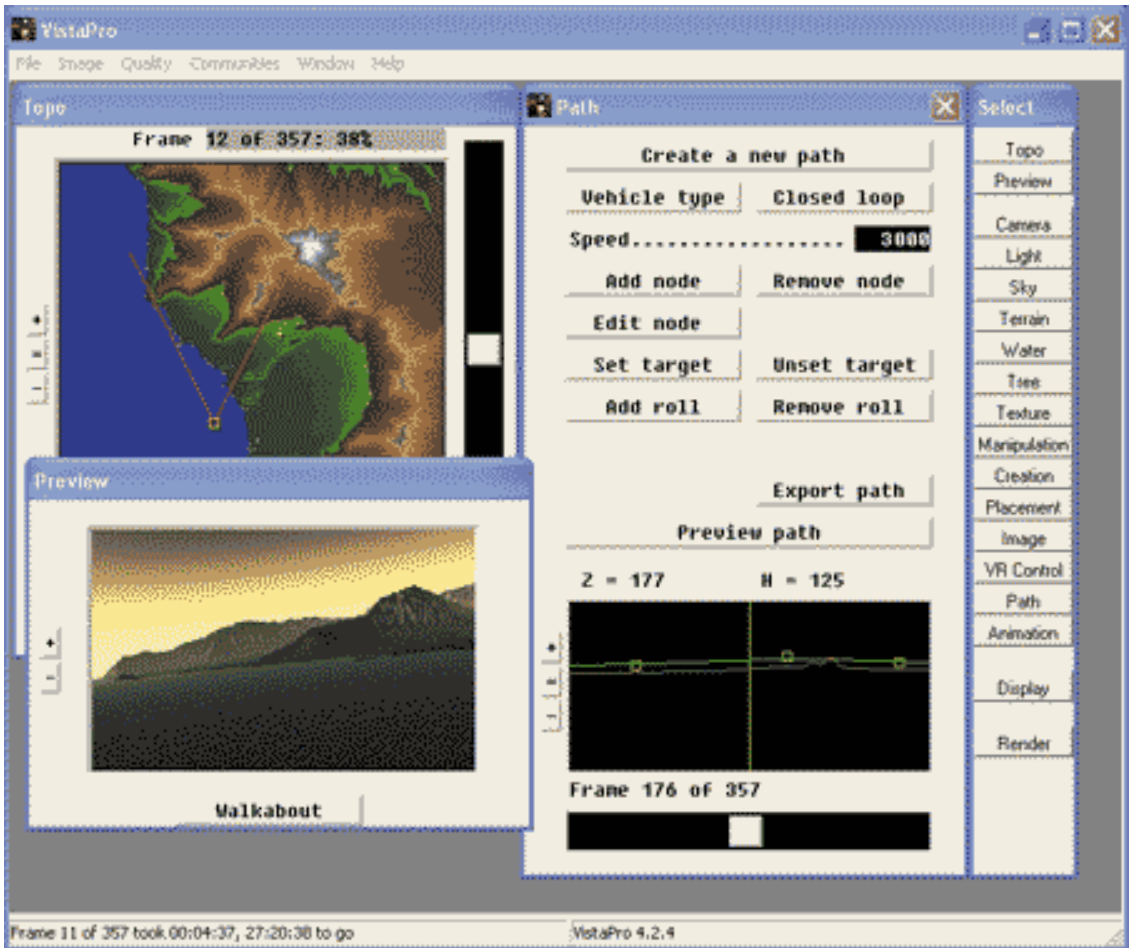
\includegraphics[scale=0.7]{vista}
 		\centering\caption{Интерфейс программы VistaPro.}
 	\end{figure}
	\subsubsection{Вывод}
	\hspace*{5mm} Не смотря на то, что существует более чем достаточное количество программного обеспечения для генерации ландшафта, характерными минусами для всего программного обеспечения является высокие требования к аппаратным ресурсам и большой объем пакетов. В своей программе я устраню эти недостатки, сделав его более гибким к системным требованиям.
	\subsection{Алгоритмы загрузки и генерации ландшафта}
	\subsubsection{Представление данных о ландшафте}
	\hspace*{5mm} Существует несколько основных принципов представления данных для хранения информации о ландшафтах:
	\begin{enumerate}
		\item использование регулярной сетки высот (или еще другое название Карта Высот - HeightMap);
		\item использование иррегулярной сетки вершин и связей, их соединяющих (т.е. хранение простой триангулизированной карты);
		\item хранение карты ландшафта, но в данном случае хранятся не конкретные высоты, а информация об использованном блоке. В этом случае создается некоторое количество заранее построенных сегментов, а на карте указываются только индексы этих сегментов.
	\end{enumerate}

	В этом проекте был выбран первый способ представления ландшафтов.
	\paragraph{Height Map:}
	 Данные представлены в виде двухмерного массива. Уже заданы две координаты (x, y - по высоте и ширине массива), и третья координата задается значением в конкретной ячейке, это высота.
	\clearpage
	\newpage
	Плюсы данного подхода:
	\begin{enumerate}
		\item простота реализации: легкость нахождения координат (и высоты) на карте, простая генерация ландшафта по карте высот или методом шума Перлина;
		\item наглядность: в любой программе просмотра графических файлов можно сразу увидеть или изменить всю информацию;
		\item скорость: благодаря конвейерной архитектуре процессора, просчет и вывод таких карт высот производится очень быстро (динамическое освещение, так как освещенность вершины напрямую зависит от расстояния от этой вершины до источника освещения).
	\end{enumerate}
	\hspace*{5mm} Минусом данного подхода является большое количество избыточных данных (особенно для поверхностей, близких к плоским).
	\\На Рисунке 4 показана визуализация данного подхода.
	\begin{figure}[h!]
		\centering
		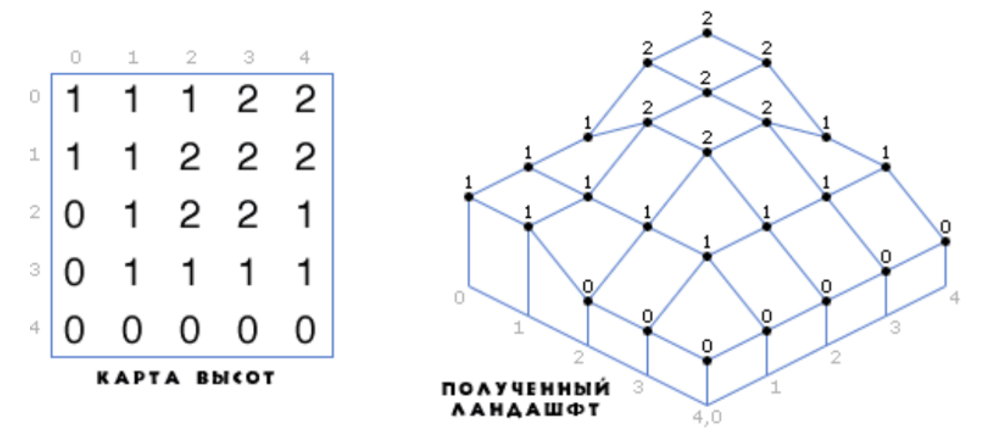
\includegraphics[scale=0.7]{heightmap}
		\centering\caption{Графическое представление метода Height Map}
	\end{figure}
	\paragraph{Иррегулярная сетка вершин и связей:}
	Еще один способ представления данных для ландшафтов про которую стоит упомянуть — иррегулярная сетка вершин и связей их соединяющих. Зачастую такие решения применяются в специализированных пакетах для игр. И хранятся в виде трехмерных моделей.
	\\ Это дает основной выигрыш по сравнению с картами высот:
	 \begin{enumerate}
	 	\item Используется значительно меньше информации для построения ландшафта. Здесь необходимо хранить только значения высот каждой вершины и связи эти вершины соединяющие. Это дает выигрыш в скорости при передаче огромных массивов информации, в процессе визуализации ландшафта.
	 \end{enumerate}
 	Но также имеются множество недостатков:
 	\begin{enumerate}
 		\item алгоритмы построения ландшафтов в основном предназначены для регулярных карт высот. Оптимизация таких алгоритмов под этот способ потребует значительных усилийа;
 		\item сложности при динамическом освещении — вершины расположены достаточно далеко друг от друга и неравномерно;
 		\item хранение, просмотр, модификация такого ландшафта также представляет сложности. При использовании карт высот достаточно применить простые и "стандартные" средства пиксельной графики. Например MS Paint. Тут же потребуются "весомые" пакеты.
 	\end{enumerate}
	Далее на Рисунке 5 показан метод иррегулярной сетки вершин и связей:
	\begin{figure}[h!]
		\centering
		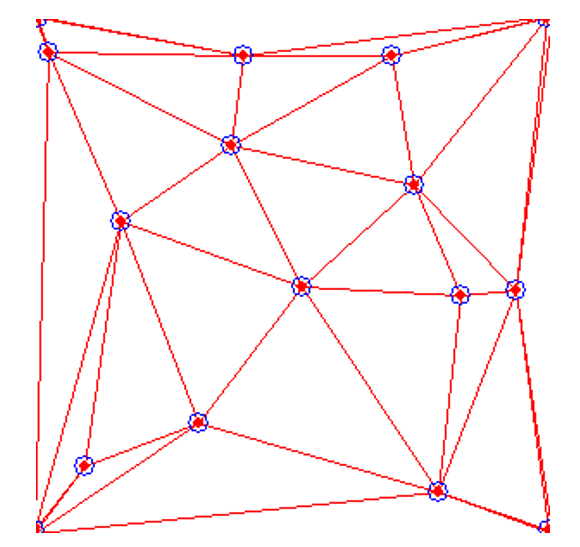
\includegraphics[scale=0.7]{irregular}
		\centering\caption{Графическое представление метода иррегулярной сетки вершин и связей}
	\end{figure}
	\subsubsection{Алгоритмы генерации рельефа}
	\paragraph{Шум Перлина:}
	При разработки данной программы возникает вопрос: откуда брать информацию для генерации карты высот? Конечно же можно просто загружать монохромное изображение и на его основе генерировать ландшафт. Но если нужно каждый раз генерировать разные карты высот (например, для компьютерных игр или демонстрационных программ, таких как эта), то на помощь приходит следующий метод на основе шума Перлина.\cite{perlin}
	\\ \hspace*{5mm} Изображение (или какой-либо другой объем) – вне зависимости от диапазона значений его элементов – полностью накрывается сеткой, представляющей диапазон вещественных чисел. Таким образом, создается шум на сетке, представляющей по всему изображению значения между 0 и 4. Каждое число порождает линию сетки, а значит, все стороны каждого квадрата последней имеют длину, равную одной единице.
	\\ \hspace*{5mm} Выбранный масштаб влияет на сложность шума. Большое число квадратов на сетке изображения создает более «плотно упакованный» шум, подобный белому шуму на экране плохо настроенного телевизора. Меньшее число квадратов на сетке порождает «клубящийся» шум, внешне похожий на облака.
	В каждой точке на сетке строится случайный вектор нормали. Это обычный двумерный вектор единичной длины, который указывает в случайном направлении в пределах каждого из квадратов. Традиционный способ создания таких векторов – организация справочной таблицы из 256 векторов, которые охватывают полный круг, и последующий случайный выбор одного из них для каждой точки на сетке. Это гарантирует распределение векторов, которые могут с равной вероятностью указывать в любом направлении. Далее для каждого пикселя изображения находится та из ячеек сетки, где он находится.
	\\ \hspace*{5mm} Таким образом, определяется значение, которое основано исключительно на данных этой ячейки. Следующий шаг – создать четыре диагональных вектора, соединяющих углы ячейки с текущим пикселем.
	\\Ниже на Рисунке 6 приведено графическое представление данного принципа:
	\clearpage
	\newpage
	\begin{figure}[h!]
		\centering
		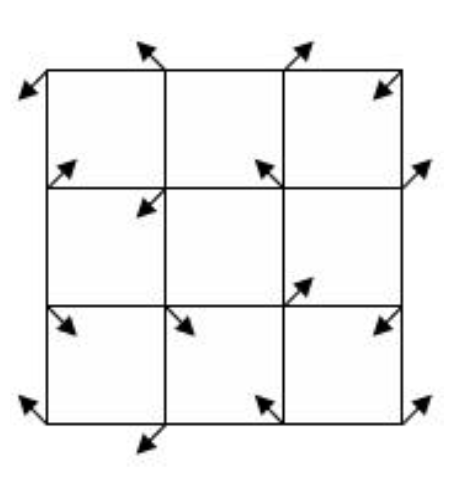
\includegraphics[scale=0.8]{perlin}
		\centering\caption{Графическое представление одного из этапов построения шума}
	\end{figure}
	 \hspace*{5mm} Каждый угол ячейки сетки теперь является базой для двух векторов – случайного единичного вектора и вектора в направлении пикселя, который необходимо построить. Для каждой пары таких векторов находиться скалярное произведение. Оно даст скалярное значение высоты каждого из углов сетки. Далее необходимо объединить эти четыре значения и найти высоту пикселя, который надо сгенерировать. Делать это можно по-разному, получая различные результаты, однако чаще всего используется взвешенная интерполяция четырех значений с учетом близости текущей позиции к каждому углу сетки.
	\\ \hspace*{5mm} Основным плюсом использования шумовой функции при генерации ландшафта является то, что нет необходимости хранить карту высот, а достаточно лишь использовать данные справочной таблицы векторов, – все остальное для восстановления конечной карты высот ландшафта сделает шумовая функция.
	\\Ниже на Рисунке 7 показан шум Перлина:
	\begin{figure}[h!]
		\centering
		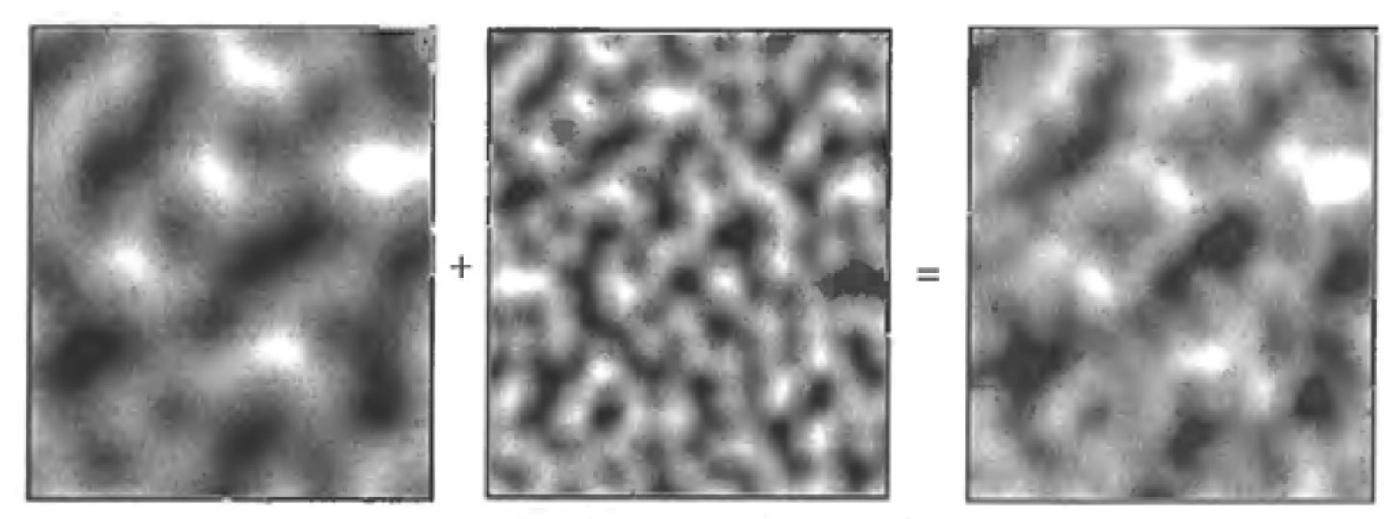
\includegraphics[scale=0.8]{perlin1}
		\centering\caption{Пример изображения шума Перлина, полученный сложением двух октав}
	\end{figure}
	\paragraph{Холмовой алгоритм:}
	Это простой итерационный алгоритм, основанный на нескольких входных параметрах.\cite{ixbt} 
	\\ Алгоритм изложен в следующих шагах:
	\begin{enumerate}
		\item создание и инициализация двухмерного массива с нулевым уровнем (все ячейки заполнены нулями);
		\item выбирается случайная точка и случайный радиус в заранее заданных пределах. Выбор этих пределов влияет на вид ландшафта - либо он будет пологим, либо скалистым;
		\item в выбранной точке "поднимается" холм заданного радиуса;
		\item возвращение ко второму шагу и так далее до выбранного количества шагов. От него будет зависеть внешний вид ландшафта;
		\item нормализация;
		\item долинизация.
	\end{enumerate}
	\hspace*{5mm} Первый, второй и четвертые шаги тривиальны, пятый и шестой шаг будет рассмотрен далее. Теперь же изучим третий шаг. Фактически холм  в этом случае половина шара, чем больше радиус - тем больше холм (и выше). Математически это похоже на перевернутую параболу:
	\begin{equation}
		z = r^2 - ((x_2 - x_1)^2 + (y_2 - y_1)^2)
	\end{equation}
	здесь ($x_1$, $y_1$) - заданная точка, r - выбранный радиус, ($x_2$, $y_2$) - высота холма.
	\\На Рисунке 8 показан одиночный холм:
	\begin{figure}[h!]
		\centering
		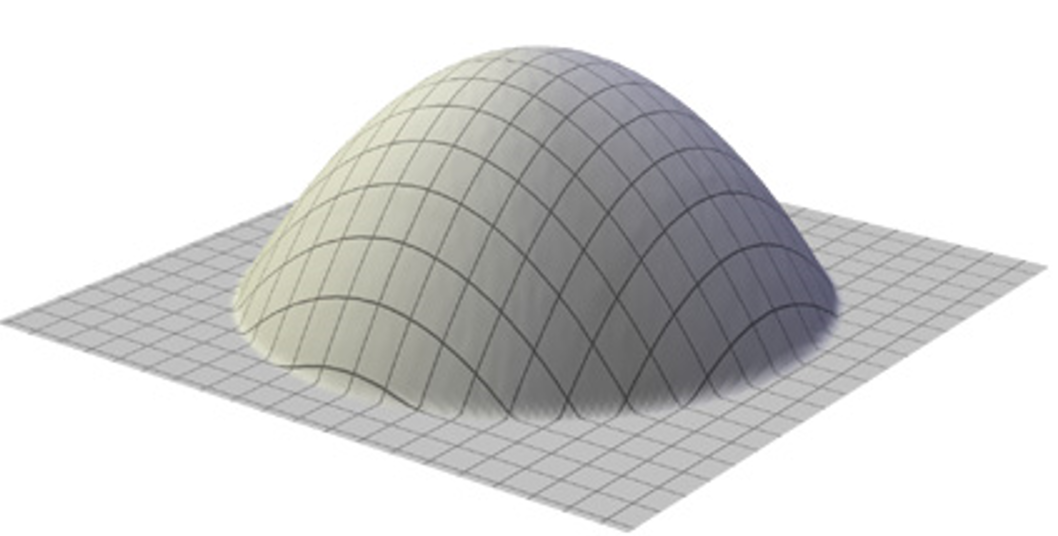
\includegraphics[scale=0.8]{holm}
		\centering\caption{Одиночный холм}
	\end{figure}
	\\ \hspace*{5mm} Чтобы сгенерировать ландшафт полностью необходимо построить множество таких холмов. Но есть еще две вещи на которые необходимо обратить внимание. Первое - игнорирование отрицательных значений высоты холма. Второе - при генерации последующих холмов лучше добавлять полученное значение для данного холма к уже существующим значениям. Это позволяет строить более правдоподобный ландшафт, нежели правильно очерченные округлые холмы. Ниже на Рисунке 9 представлен ландшафт при большом количестве итераций:
	\clearpage
	\newpage
	\begin{figure}[h!]
		\centering
		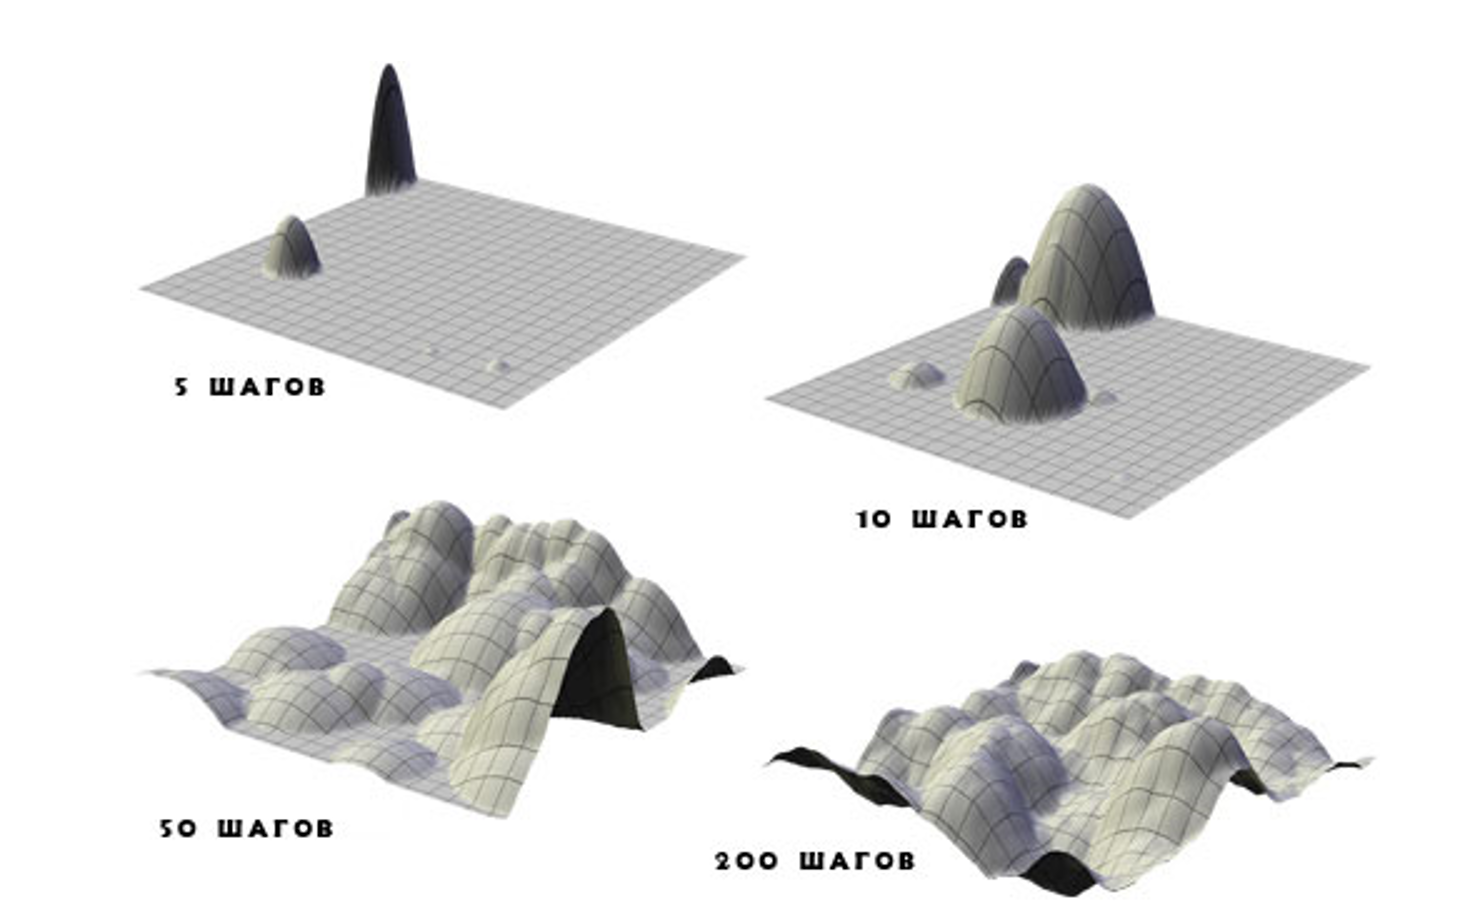
\includegraphics[scale=0.8]{steps}
		\centering\caption{Ландшафт при большом количестве итераций}
	\end{figure}
	
	\textbf{Нормализация ландшафта}
	\\ \hspace*{5mm}При генерации значений для ландшафта не учитывались выходы этих значений за некоторые пределы (например, если ландшафт будет храниться в монохромной картинке, то необходимо, чтобы все значения находились в пределе от 0 до 256). Для этого необходимо произвести нормализацию значений. Математически нормализация — это процесс получения значений из одного предела, и перевод его в другие пределы. Вот как это выглядит графически на Рисунке 10:
	\begin{figure}[h!]
		\centering
		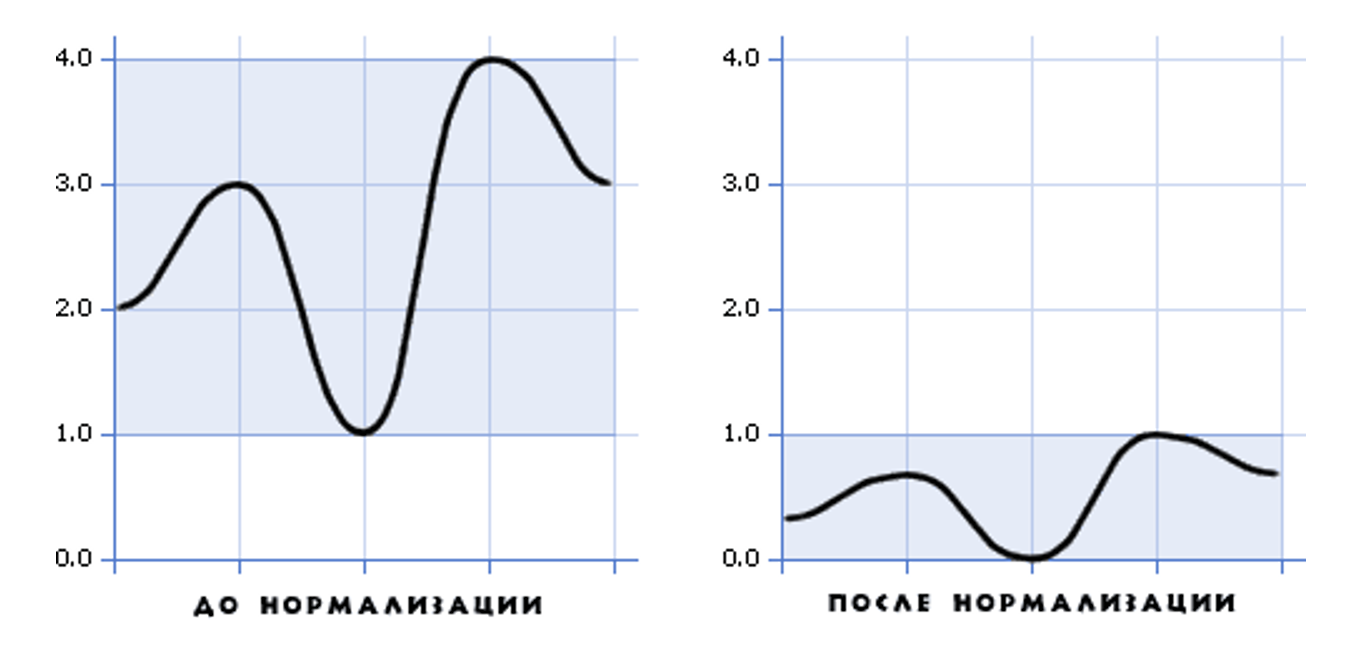
\includegraphics[scale=0.9]{normal}
		\centering\caption{Разница использования <<Нормализации>>}
	\end{figure}
	\\ Чтобы это сделать произведем следующие действия:
	 \begin{enumerate}
	 	\item сперва проходим по всему массиву и запоминаем наибольшее и наименьшее значения;
	 	\item после этого производится нормализация конкретных значений в пределах от 0 до 1.Формула  выглядит так:
	 \end{enumerate}
  	\begin{equation}
  		z = \frac{z - min}{max - min}
  	\end{equation}
  \clearpage
  \newpage
  \textbf{Долинизация ландшафта}
  \\ \hspace*{5mm} Данный ландшафт уже можно использовать, но если присмотреться, то в нем достаточно мало долин. Склоны холмов излишне крутые, необходимо сделать их более пологими. Идея <<Долинизации>> состоит в следующем - взять от каждого значения квадратный корень. Это в большей степени влияет на средние значения, практически не затрагивая минимумов и максимумов. Графически это выглядит так как на Рисунке 11:
  \begin{figure}[h!]
  	\centering
  	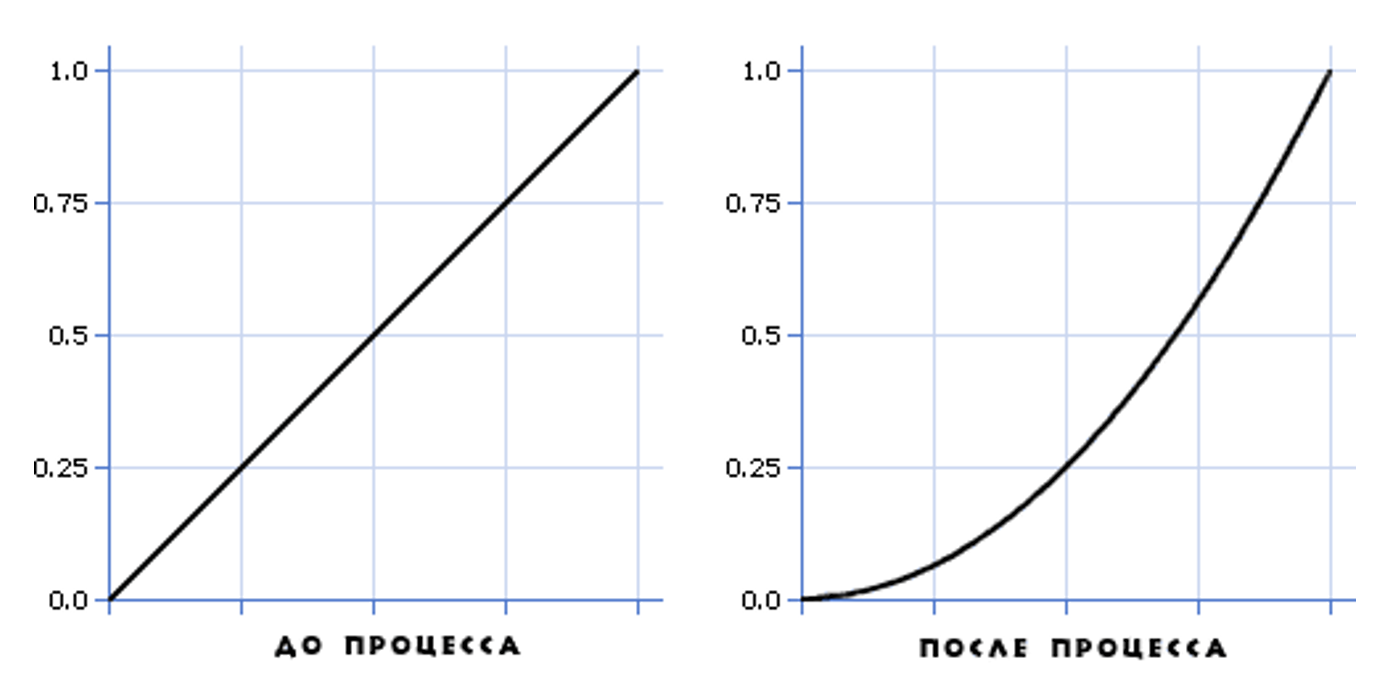
\includegraphics[scale=0.9]{dol}
  	\centering\caption{Разница использования <<Долинизации>>}
  \end{figure}
	\\На Рисунке 12 можно увидет преобразования ландшафта после <<Долинизации>> и <<Нормализации>>:
	\begin{figure}[h!]
		\centering
		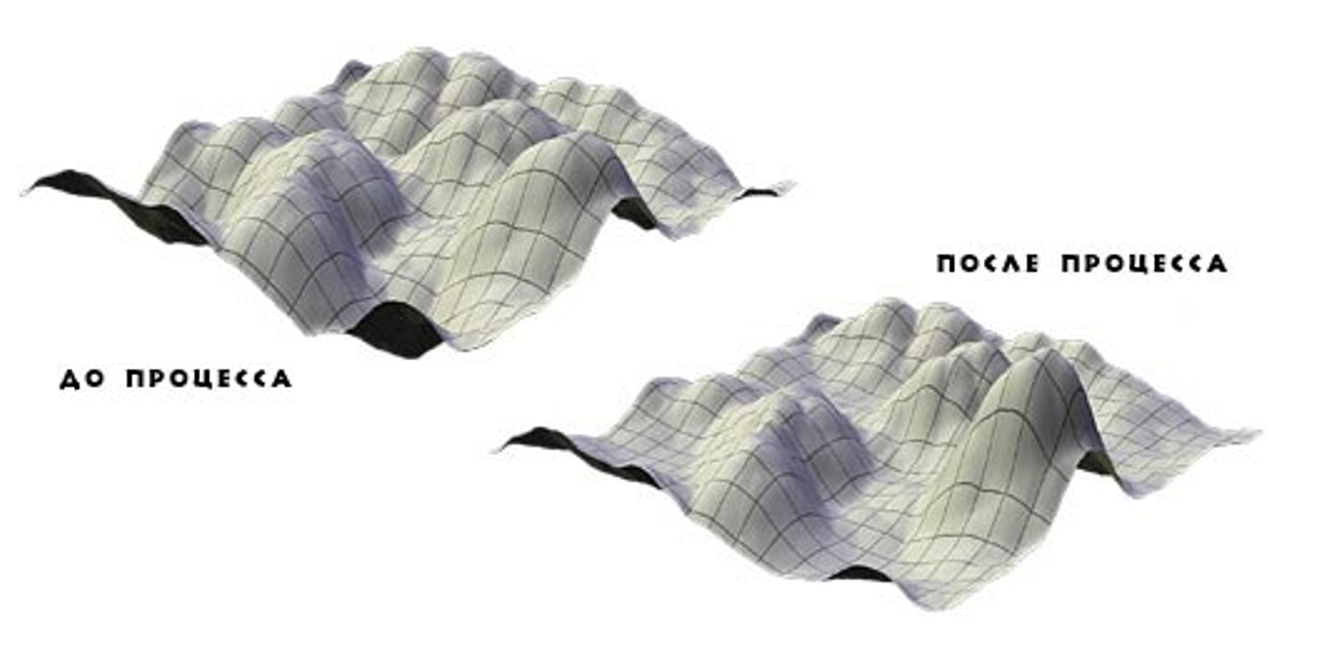
\includegraphics[scale=0.9]{diff}
		\centering\caption{Разница ландшафтов при использования <<Долинизации>> и <<Нормализации>> }
	\end{figure}
	\\ \hspace*{5mm}В основном, рассмотренные выше алгоритмы предназначены для создания простого холмистого или гористого ландшафта. Но существуют и другие типы ландшафтов. Например, острова, озерные ландшафты. Их можно реализовать достаточно просто:
	\begin{enumerate}
		\item создание простого, достаточно холмистого ландшафта;
		\item перемещение уровня воды вверх или вниз.
	\end{enumerate}
	\clearpage
	\newpage
	\hspace*{5mm}Так как уже было сказано выше, что ландшафт будет генерироваться двумя видами (остров и холмы). Ввиду того, что холмы уже рассмотрены. Необходимо понять, как правильно создать остров, чтобы он был реалистичным.
	\\ \hspace*{5mm} Во многих случаях используется уже рассмотренный алгоритм для генерации ландшафтов. Но иногда необходимо сгенерировать острова, или остров. В этом поможет слегка модифицированный алгоритм.
	В исходном алгоритме выбиралась центральная точка случайным образом, и она могла располагаться в любой части ландшафта. Теперь же необходимо, чтобы холмы были расположены ближе к центру.
	\\ \hspace*{5mm} Чтобы сделать это, вводятся две переменные (которые потом будем случайным образом изменяться), назовем их расстояние и угол. Расстояние будет означать, как далеко от центра находится центральная точка для одиночного холма. Оно может изменяться от ноля (прямо по центру карты высот) до половины величины карты высот минус радиус холма. Это позволит избежать ситуаций пересечения холмов с краем карты высот. Угол будет показывать, в каком направлении от центра нужно будет поставить холм. Изменяется угол будет в пределах от 0 до двух Пи. Используя эти два значения, можно получить значения (x, y) для центральной точки конкретного холма и использовать их как и в простом алгоритме.
	\\ Ниже представлен способ получения значений для $x$ и $y$:
	\begin{equation}
		\theta = random(0, 2\pi)
	\end{equation}
	\begin{equation}
		distance = random(0, \frac{size}{2} - radius)
	\end{equation}
	\begin{equation}
		x = \frac{size}{2} + \cos(\theta) * distance
	\end{equation}
	\begin{equation}
		y = \frac{size}{2} + \sin(\theta) * distance
	\end{equation}
	здесь $size$ - размер карты высот, $distance$ - расстояние, $\theta$ - угол. Важно, чтобы радиус был меньше половины размера карты высот.
	\\Поработав с этими величинами, можно получить довольно прилично выглядящий остров. На Рисунке 13 показан этот остров:
	\clearpage
	\newpage
	\begin{figure}[h!]
		\centering
		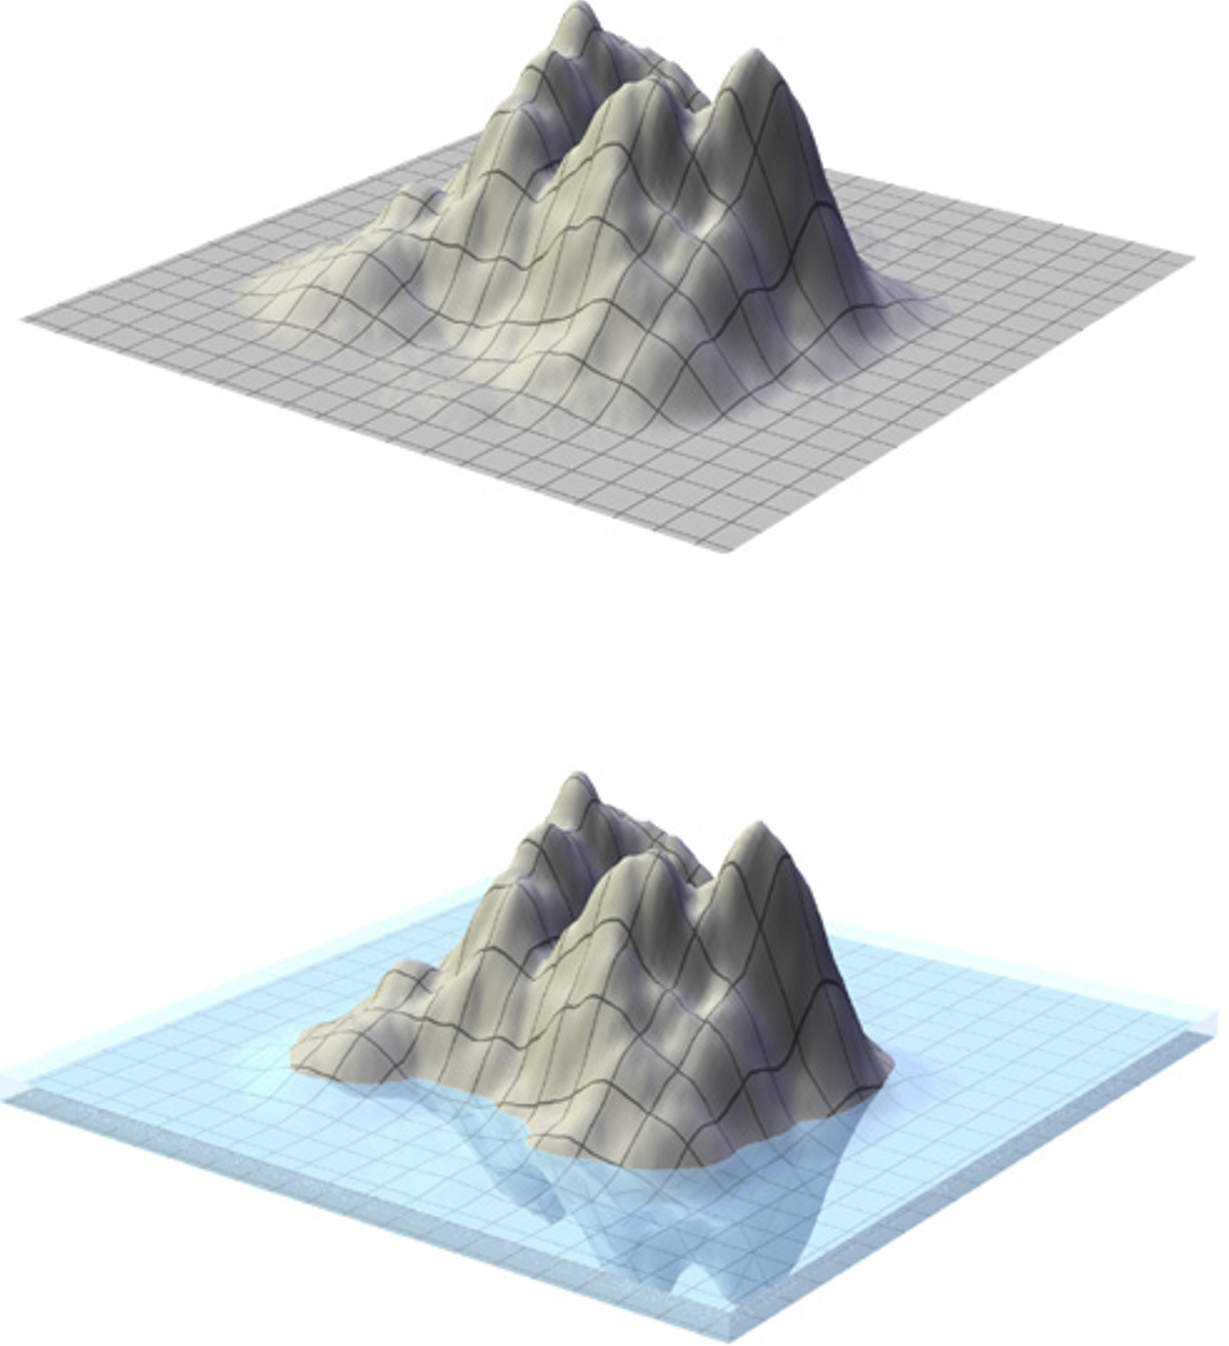
\includegraphics[scale=0.9]{two}
		\centering\caption{Получение из обычного холма остров}
	\end{figure}
	 Выше были разобраны некоторые алгоритмы построения карт высот для ландшафтов. Рассмотрим еще некоторые сопутствующие операции:
	\begin{enumerate}
		\item сглаживание (или размытие). Низкочастотный фильтр для уменьшения эффектов угловатости. При многократном применении позволяет добиться очень гладких очертаний ландшафта;
		\item превращение гористой местности в холмистую. Различия выделяются по очертанию вертикальных разрезов у вторых более пологие края;
		\item создание пляжей и отмелей в случае с островами и берегами. Для этого места соприкосновения с водой сглаживают. Хотя могут существовать и скалистые пляжи и просто скалы.
	\end{enumerate}
	\subsubsection{Вывод}
	\hspace*{5mm} В данном разделе были рассмотрены алгоритмы представления данных и генерации ландшафта. Из перечисленных выше алгоритмов предатсвления данных был выбран алгоритм использования регулярной сетки высот, так как является самым популярным и простым в реализации методом.
	\subsection{Алгоритмы визуализации ландшафта и окружающей среды}
	\subsubsection{Использование карт освещенности}
	 \hspace*{5mm} В широком смысле \textit{карта освещения} – это структура данных, хранящая информацию об освещенности (яркости) поверхностей трехмерной сцены. Карты освещения рассчитываются предварительно для неподвижных объектов и позволяют ускорить рисование освещенной сцены. Сейчас под картами освещения чаще всего подразумевают одну из их разновидностей – текстурные карты освещения. Они представляют собой изображения, накладываемые при рисовании «поверх» основных текстур; при этом яркость точки на карте освещения используется для модуляции яркости точки основной текстуры. Этот процесс продемонстрирован на Рисунке 14:
	 \begin{figure}[h!]
	 	\centering
	 	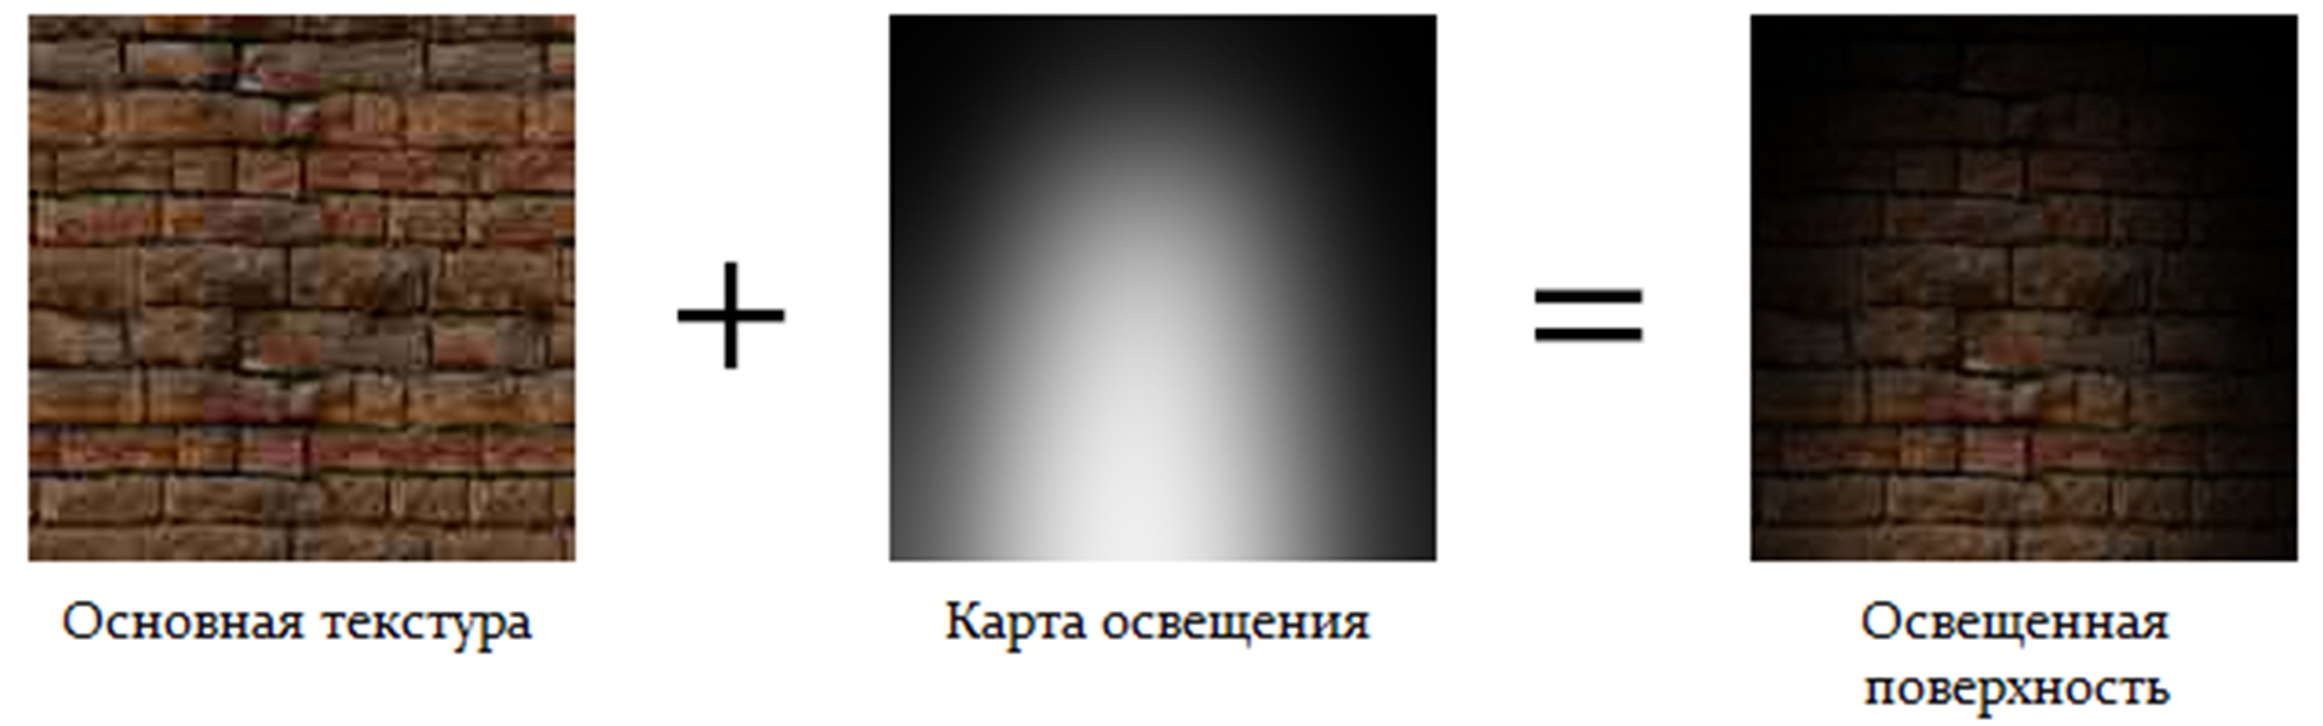
\includegraphics[scale=0.6]{osv}
	 	\centering\caption{Использование карты освещенности}
	 \end{figure}
 	\\ \textbf{Вычисление результирующего цвета}
 	\\$R = R_{text} * R_{light}$
 	\\$G = G_{text} * G_{light}$
 	\\$B = B_{text} * B_{light}$
 	\\ \hspace*{5mm} Значение компонентов цвета лежат в диапазоне [0, 1].
 	Если карта освещенности будет полностью белой, то результирующая текстура будет такой же, как и основная текстура (компоненты везде домножаются на 1, так как белый цвет это R = 1, G = 1, B = 1)
 	если карта освещенности будет полностью черной, то результирующая текстура тоже черной (компоненты везде домножаются на 0, так как черный цвет это R = 0, G = 0, B = 0), что соответствует отсутствие источников освещения.\cite{rgb}
 	\subsubsection{Наложение текстур}
 	\hspace*{5mm}Текстуры позволяют увеличить детализированность изображения, не добавляя в сцену дополнительную геометрию, и поэтому широко распространены в трехмерной графике .
 	Как правило, трехмерная модель, созданная в пакете трехмерного моделирования, содержит не только информацию о геометрии, но и текстурные координаты – пары чисел U и V, указывающие на точку текстуры. Текстурные координаты задаются в вершинах граней, и задача наложения текстур сводится к интерполяции текстурных координат U и V по всем точкам грани.
 	\\В аффинном текстурировании используется линейная интерполяция:
 	\begin{equation}
 		u_\alpha = (1 - \alpha)u_0 + \alpha u_1
 	\end{equation}
 	\hspace*{5mm} Здесь $u_0$ и $u_1$ – значения текстурной координаты U, заданные на концах некоторого отрезка. Точно такая же формула используется для координаты V.
 	Этот метод работает быстро, но дает некорректные результаты для граней, расположенных под углом к экрану, так как при интерполяции не учитываются значения глубины точек.
 	\\ \hspace*{5mm} Перспективно-корректное текстурирование, как следует ожидать из названия, дает корректные результаты для произвольных граней благодаря дополнительной интерполяции глубины точек:
 	\begin{equation}
 		u_\alpha = \frac{(1-\alpha)\frac{u_0}{z_0} + \alpha\frac{u_1}{z_1}}{(1-\alpha)\frac{1}{z_0} + \alpha\frac{1}{z_1}}
 	\end{equation}
 	\hspace*{5mm} Здесь $z_0$, $z_1$ – глубины концов отрезка, на котором проводится интерполяция. Ниже на рисунке 15 представлено сравнение методов текстурирования:
 	\begin{figure}[h!]
 		\centering
 		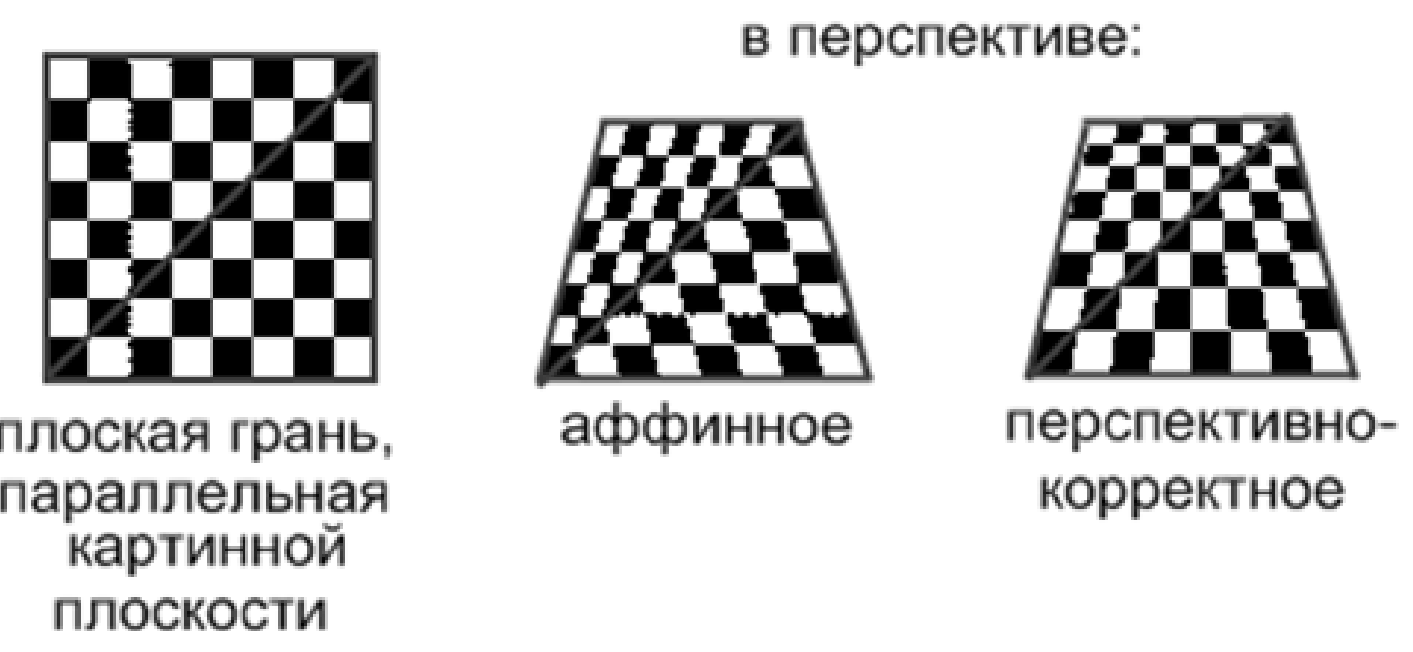
\includegraphics[scale=0.7]{tekstr}
 		\centering\caption{Сравнение методов текстурирования}
 	\end{figure}
 	\subsubsection{Смешивание текстур}
 	\hspace*{5mm} Прозрачность реализуется с помощью специального режима смешения цветов (\textit{blending}). Алгоритм смешения комбинирует цвета так называемых входящих пикселей с цветами соответствующих пикселей, уже хранящихся в буфере. Для смешения используется четвертая компонента цвета – альфа-компонента, поэтому этот режим называют еще альфа-смешиванием. Программа может управлять интенсивностью альфа-компоненты точно так же, как и интенсивностью основных цветов, т.е. задавать значение интенсивности для каждого пикселя или каждой вершины примитива. Расчет результирующего цвета каждого пикселя:
 		\begin{equation}
 		res = c_{src}*k_1+c_{dst}*k_2
 	\end{equation}
	\\ \hspace*{5mm} Параметр $src$ определяет, как получить коэффициент $k_1$ исходного цвета пикселя, a $dst$ задает способ получения коэффициента$k_2$ для цвета в буфере кадра. Параметр $c_{src}$ – цвет исходного пикселя, $c_{dst}$ – цвет пикселя в буфере кадра ($res, k_1, k_1, c_{src}, c_{dst}$ – четырехкомпонентные RGBA-векторы).
	\\ \hspace*{5mm}Если в сцене есть несколько прозрачных объектов, которые могут перекрывать друг друга, корректный вывод можно гарантировать только в случае выполнения следующих условий:
	\begin{enumerate}
		\item все прозрачные объекты выводятся после непрозрачных;
		\item при выводе объекты с прозрачностью должны быть упорядочены по уменьшению глубины, т.е. выводиться, начиная с наиболее отдаленных от наблюдателя.
	\end{enumerate}
	\subsubsection{Мипмапы}
	\hspace*{5mm}Мипмапы или Мип-карты  — предрассчитанный, оптимизированный набор изображений связанных с одной текстурой и предназначенный для увеличения скорости рендеринга и улучшения качества изображения.\cite{mm}
	\\ \hspace*{5mm}Каждое следующее изображение в наборе вдвое меньше предыдущего. То есть самое первое имеет размер равный размеру текстуры, второе вдвое меньший, третье — вчетверо и так далее до размера 1х1 тексель. На Рисунке 16  представлен пример Мип-карты:
	\begin{figure}[h!]
		\centering
		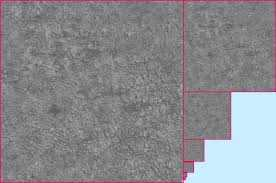
\includegraphics[scale=0.8]{mipmap}
		\centering\caption{Пример Мип-карты}
	\end{figure}
	\\ \hspace*{5mm} Смысл такого вот пред рассчитанного набора состоит в том, что при текстурировании будет выбираться изображение с наиболее подходящим размером.
	Предположим, что на модель натянута текстура размером 512х512. Модель стоит далеко от камеры и геометрические размеры на экране у нее малы (скажем 3 пикселя)
	При отключенном мипмапинге видеокарте придётся выбирать, какой тексель из большой текстуры будет использован для расчёта цвета точки. Этот выбор может меняться при изменении ракурса камеры, что приведёт к мерцанию объектов вдали.
	\\ \hspace*{5mm} При включенном мипмапинге видеокарта выберет более подходящий размер текстуры, и будет производить выборку из него, что избавит нас от артефактов изображения. Использование мипмапинга также повышает быстродействие, так как более эффективно используется текстурная кэш-память видеокарты, и меньше данных приходиться передавать по шине.
	\newline\\ Генерацию мип-уровней можно сделать несколькими способами:
	\begin{enumerate}
		\item указать видеокарте сгенерировать мип-уровни. Качество не будет очень хорошим, так как для генерации будет использоваться простой Box фильтр;
		\item генерировать мипмапы самому, воспользовавшись пакетами для редактирования изображений;
		\item отрисовать все мип-уровни вручную.
	\end{enumerate}
	\hspace*{5mm} При применении \textit{Билинейной фильтрации} или \textit{Трилинейной фильтрации} с мипмапингом можно получить более размытые текстуры на поверхностях вдали или под углом. 
	\paragraph{Билинейная фильтрация} - процесс извлечения нескольких пикселей исходной текстуры с последующим усреднением их значений для получения окончательного значения пикселя. Понятие «билинейная фильтрация», точно так же, как и сходное понятие «трилинейная фильтрация», применимо только к двумерным текстурам. Для трехмерных, например, данное понятие неприменимо, а понятие трилинейной фильтрации имеет совершенно другое значение. Пример исходного кода функции билинейной фильтрации.
	\paragraph{Трилинейная фильтрация} - усовершенствованный вариант билинейной фильтрации. Цвет пикселя высчитывается как средневзвешенное восьми текселей: по четыре на двух соседних MIP-текстурах. В случае, если формулы MIP-текстурирования дают самую крупную или самую маленькую из MIP-текстур, трилинейная фильтрация вырождается в билинейную.
	
	 \vspace{0.8mm} \hspace*{5mm} MIP-текстурирование, повышая чёткость изображения и процент попаданий в кэш на дальних расстояниях, имеет серьёзный недостаток: ясно видны границы раздела между MIP-уровнями. Трилинейная фильтрация позволяет исправить этот недостаток ценой некоторого снижения резкости текстур.
	 \subsubsection{Алгоритм Z-буфера}
	 \hspace*{5mm}Это один из простейших алгоритмов удаления невидимых поверхностей. Работает этот алгоритм в пространстве изображения. Идея z-буфера является простым обобщением идеи о буфере кадра. Буфер кадра используется для запоминания атрибутов (интенсивности) каждого пикселя в пространстве изображения, z-буфер – это отдельный буфер глубины, используемый для запоминания координаты z, или глубины каждого видимого пикселя в пространстве изображения.\cite{zbuff}
	 \\ \hspace*{5mm} Главное \textit{преимущество} алгоритма – его простота. Кроме того, этот алгоритм решает задачу об удалении невидимых поверхностей и делает тривиальной визуализацию пересечений сложных поверхностей. Сцены могут быть любой сложности. Поскольку габариты пространства изображения фиксированы, оценка вычислительной трудоемкости алгоритма не более чем линейна. Поскольку элементы сцены или картинки можно заносить в буфер кадра или в z-буфер в произвольном порядке, их не нужно предварительно сортировать по приоритету глубины. Поэтому экономится вычислительное время, затрачиваемое на сортировку по глубине. При этом, алгоритм z-буфера, будучи реализованный аппаратно, является самым быстрым алгоритмом удаления невидимых поверхностей.
	 \\ \hspace*{5mm} Основной недостаток алгоритма – большой объем требуемой памяти. Другой недостаток алгоритма z-буфера состоит в трудоемкости и высокой стоимости устранения лестничного эффекта, а также реализации эффектов прозрачности и просвечивания. 
	 \\ \hspace*{5mm} При визуализации изображения, как пиксельная информация, так и глубина усредняются. В этом методе требуются очень большие объемы памяти. Например, изображение размером 512х512х24 бита, использующее z-буфер размером 20 бит на пиксель, разрешение которого повышено в 2 раза по осям х и у, и на котором устранена ступенчатость методом равномерного усреднения, требует почти 6 МБ памяти.
	 \subsubsection{Вывод}
	 \hspace*{5mm} Здесь были расммотрены алгоритмы визуализации ландшафта и окружающей среды. Были показаны плюсы и минусы использования мип-карты. Представлены решения проблем полученных при использовании мип-уровней. Были рассмотрены способы увеличения скорости показана изображения.
	 \subsection{Выводы из аналитической части}
	 \hspace*{5mm} В данном разделе были представлены алгоритмы загрузки данных о ландшафте. Были предасталены преимущества и недостатки этих методов. Также было подробно описанот про порядок визуализации ландшафта и окружающей среды. Побробная схема реализация всх этих алгоритмов будет представлена в следующем разделе. 
%\end{flushleft}
\clearpage
\newpage
\section{Конструкторская часть}
%\begin{flushleft}
	 \hspace*{5mm} В данном разделе представлены подробное описание процесса освещения, рассчета теней, а также схемы алгоритмов указанных в аналитической части.
	 \subsection{Разработка алгоритмов}
	 В данном пункте будут рассмотрены схемы следующих алгоритмов:
	 \begin{enumerate}
	 	\item Холмовой алгоритм;
	 	\item Алгоритм Z-буфера.
	 \end{enumerate}
	На Рисунках 17 и 18 представлены схемы алгоритмов z-буфера и  холмового алгоритма:
	\clearpage
	\newpage
	\begin{figure}[h!]
		\centering
		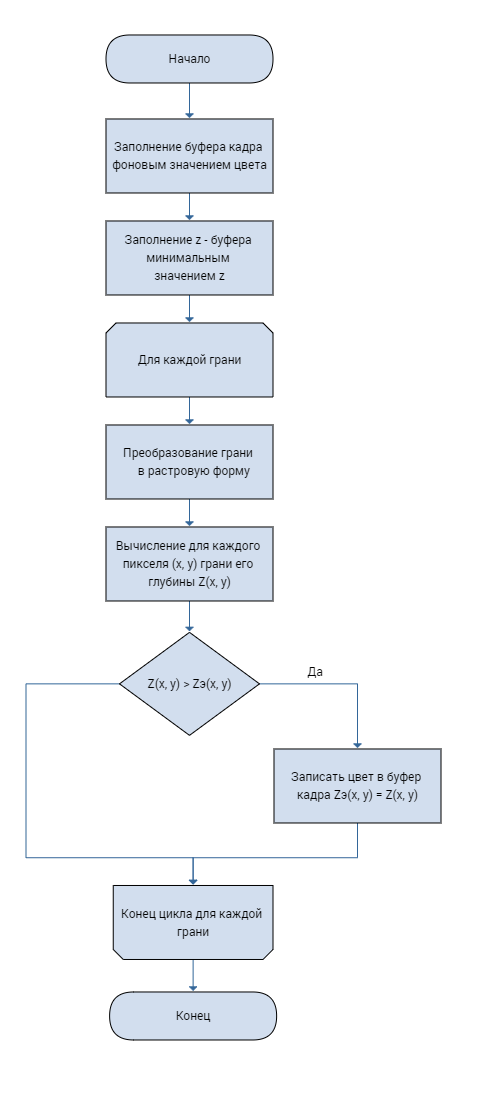
\includegraphics[scale=0.6]{z-buff}
		\centering\caption{Схема алгоритма Z-буфера}
	\end{figure}
	\clearpage
	\newpage
	\begin{figure}[h!]
		\centering
		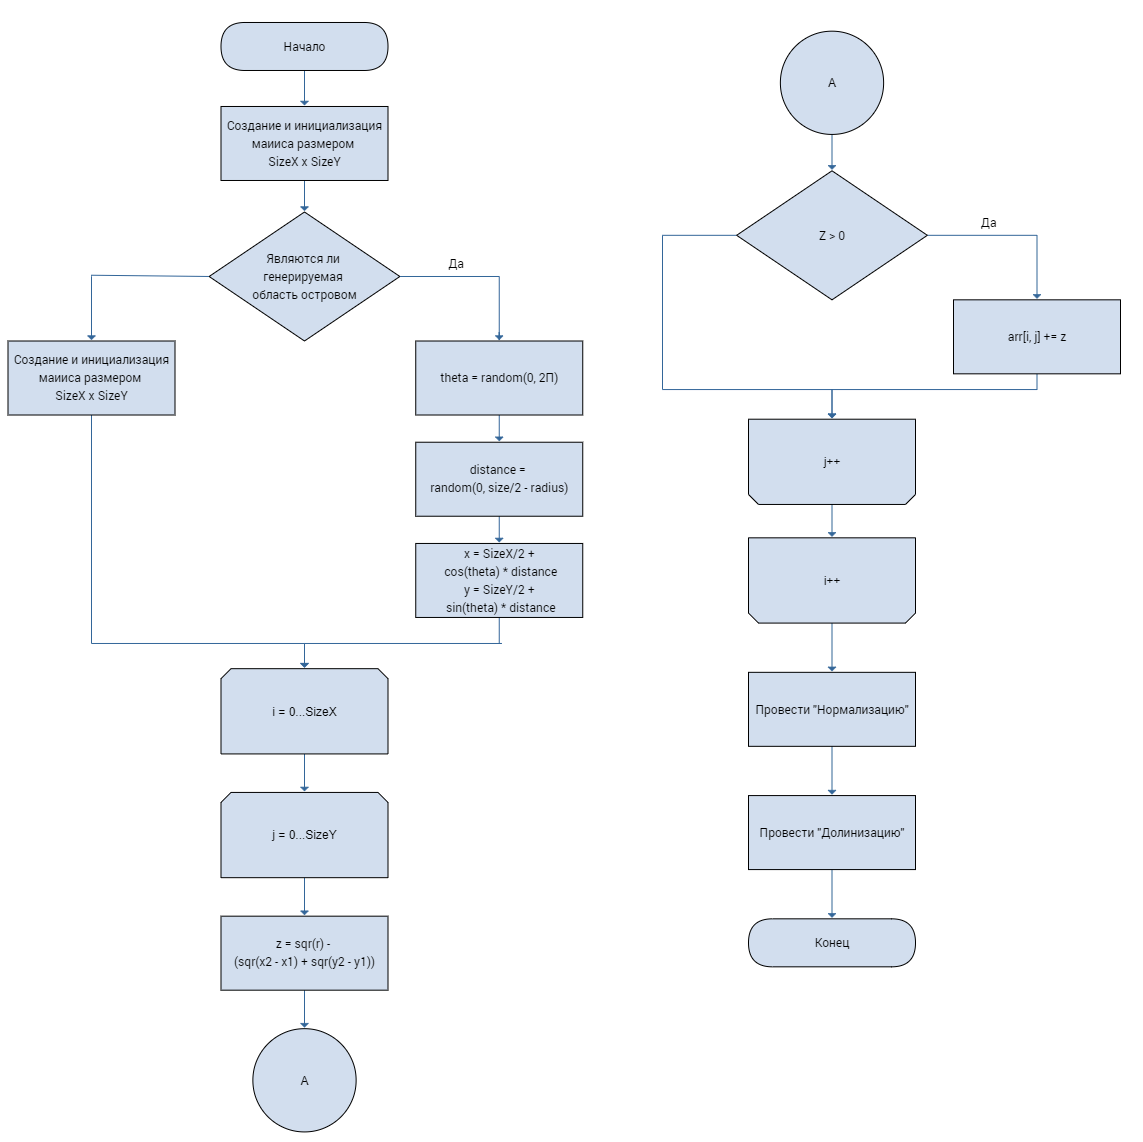
\includegraphics[scale=0.4]{schema_hill}
		\centering\caption{Схема холмового алгоритма}
	\end{figure}
	\subsection{Освещение}
	\hspace*{5mm} В любом трёхмерном приложении использование какой-либо модели освещения всегда придаёт реалистичность обрабатываемой сцене. Как правило, в неё включается закон, по которому рассчитывается освещённость точки в пространстве, и метод закраски освещённого многоугольника. От выбора той или иной модели освещения зависит качество изображения, построенного компьютером, и скорость работы программы.
	\\ \hspace*{5mm} Обычно освещённость некоторой точки, принадлежащей грани в пространстве, складывается из рассеянной освещённости и диффузного отражения — потока света, отражающегося от поверхности объекта. Иногда к ним добавляют зеркальное отражение — поток света, отражающийся от внешней поверхности объекта под тем же углом, под которым он падал на эту поверхность. Однако в данной работе зеркальное отражение света не учитывается, так предварительно производится расчет карты освещенности, которая затем модулируется с текстурой и накладывается на трехмерный объект, а при расчете зеркальной компоненты света учитывается положение наблюдателя, которое может быть различным в определенный момент времени (нужно будет пересчитывать карту освещенности заново, что недопустимо). Кроме того, расчёт интенсивности зеркального отражения, например по модели Фонга, требует немалых вычислительных затрат. Для него требуется рассчитывать угол между вектором наблюдения и вектором отражения и возводить косинус этого угла в некоторую степень, зависящую от свойств поверхности.
	\\ \hspace*{5mm} Диффузное отражение присуще матовым поверхностям. Матовой можно считать такую поверхность, размер шероховатостей которой настолько велик, что падающий луч рассеивается неравномерно во все стороны. Такой тип отражения характерен, например, для гипса, песка, бумаги. Диффузное отражение описывается законом Ламберта, согласно которому интенсивность отраженного света пропорциональна косинусу угла между направлением на точечный источник света и нормалью к поверхности(10).
	\begin{figure}[h!]
		\centering
		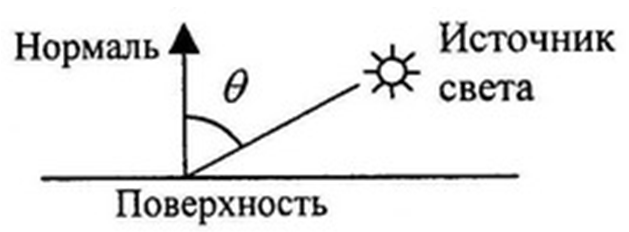
\includegraphics[scale=0.6]{norm}
		\centering\caption{Матовая поверхность}
	\end{figure}
	\begin{equation}
		I_d = IK_d\cos\theta
	\end{equation}
	Здесь $I_d$- интенсивность источника света, $K_d$ - коэффициент, который учитывает свойства материала поверхности. Интенсивность отраженного света не зависит от расположения наблюдателя.
	\\ \hspace*{5mm}Матовая поверхность имеет свой цвет. Наблюдаемый цвет матовой поверхности определяется комбинацией собственного цвета поверхности и цвета излучения источника света (в данной работе цвет излучения источника считается белым, поэтому учитывается только цвет поверхности).
	\\ \hspace*{5mm}Для точечного источника света можно еще усовершенствовать модель отражения, если учесть, что энергия уменьшается пропорционально квадрату расстояния и пропорционально расстоянию. 
	\\ \hspace*{5mm}Кроме того, в данной программе вместо интенсивности света используется расширенная величина цвет света, которая состоит из трех компонент ($R, G, B$)	
	\\ \hspace*{5mm}Итак, цвет в данной точке для одного источника направленного освещения рассчитывается по следующей формуле:
	\begin{equation}
		I_{reflection}= I_{light}K_d\cos\theta
	\end{equation}
	Для точечного источника света:
	\begin{equation}
		I_{reflection}= \frac{I_{light}}{c_1 + c_2d + c_3d^2}K_d\cos\theta
	\end{equation}
	\\ $I$ - интенсивность источника света($R, G, B$).
	\\ $K_d$ - способность материала отражать диффузный свет (тоже имеет $R, G, B$).
	\\ $d$ - расстояние от источника света до рассматриваемой точки поверхности, 
	$c_1, c_3, c_3$ – произвольные коэффициенты угасания, которые находятся эмпирическим путем
	\\ Для определения косинуса угла между вектором нормали к поверхности и вектором, определяющим положение источника света в пространстве, следует воспользоваться скалярным произведением. Пусть имеется вектор нормали $N(X_N, Y_N, Z_N)$ и две точки – $P(X_P, Y_P, Z_P)$ , принадлежащая поверхности, и  $L(X_L, Y_L, Z_L)$, определяющая положение источника. Вектор, направленный от точки поверхности к источнику света, имеет следующие координаты:  $V(X_L - X_P, Y_L - Y_P, Z_L - Z_P)$. Тогда
	\begin{equation}
		N * V = |N||V|\cos\theta
	\end{equation}
	\begin{equation}
		|N| = \sqrt{X_N^2 + Y_N^2 + Z_N^2}
	\end{equation}
	\begin{equation}
		|V| = \sqrt{(X_L - X_P)^2 + (Y_L - Y_P)^2 + (Z_L - Z_P)^2}
	\end{equation}
	Расспишем (13) используя (14) и (15):
	\begin{equation}
		N * V = X_NX_V + Y_NY_V + Z_NZ_V
	\end{equation}
	Следовательно угол равен:
		\begin{equation}
		\cos\theta = \frac{X_NX_V + Y_NY_V + Z_NZ_V}{|N||V|}
	\end{equation}
	Однако в программе используются, как правило, единичные вектора нормалей, что в данном случае позволяет уменьшить количество требуемых вычислений. В итоге:
	\begin{equation}
		\cos\theta = \frac{X_N(X_L - X_P) + Y_N(Y_L - Y_P) + Z_N(Z_L - Z_P)}{|V|}
	\end{equation}
	Или более развернуто,
	\begin{equation}
		\cos\theta = \frac{X_N(X_L - X_P) + Y_N(Y_L - Y_P) + Z_N(Z_L - Z_P)}{\sqrt{(X_L - X_P)^2 + (Y_L - Y_P)^2 + (Z_L - Z_P)^2}}
	\end{equation}
	\subsection{Модель освещения Фонга и просчет теней}
	\hspace*{5mm}При использовании метода Фонга для определения цвета в каждой точке интерполируются не интенсивности отраженного света, а векторы нормалей\cite{fong}.
	Последовательность действий такова:
	\begin{enumerate}
		\item определяются нормали к граням;
		\item по нормалям к граням определяются усредненные нормали в вершинах. В каждой точке закрашиваемой грани определяется интерполированный вектор нормали;
		\item по направлению векторов нормали определяется цвет точек грани в соответствии с принятой моделью отражения цвета.
	\end{enumerate}
	 \hspace*{5mm} Как уже было сказано, метод заключается в интерполяции вектора нормали. Для интерполяции будут использоваться векторы  $N_a^{`}$, $N_b^{`}$, $N_c^{`}$, исходящие из начала координат плоскости проецирования и параллельными соответствующим нормалям $N_a$, $N_b$, $N_c$ в вершинах $a, b, c$.
	 \clearpage
	 \newpage
	 \begin{figure}[h!]
	 	\centering
	 	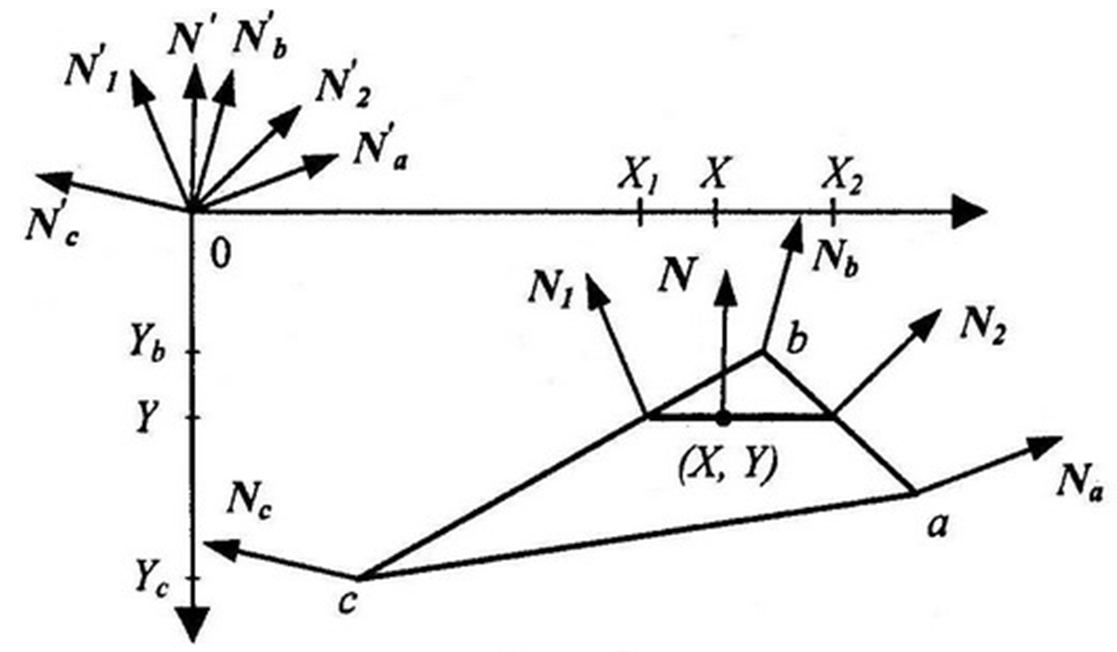
\includegraphics[scale=0.9]{lines}
	 	\centering\caption{Графическое представление векторов для интерполяции}
	 \end{figure}
 	Нахождение $N_1^{`}$ и $N_2^{`}$ и производится следующим образом:
 	\newline \newline  \hspace*{3cm} $N_1^`=\begin{pmatrix} X_{N1}\\Y_{N1}\\Z_{N1}\end{pmatrix} = 
 	\begin{pmatrix} X_{Nb} + \frac{(X_Nc - X_Nb)(Y - Y_b)}{Y_c -Y_b}\\
 		Y_{Nb} + \frac{(Y_Nc - Y_Nb)(Y - Y_b)}{Y_c -Y_b}\\
 		Z_{Nb} + \frac{(Z_Nc - Z_Nb)(Y - Y_b)}{Y_c -Y_b}\end{pmatrix}$

	\vspace*{1cm}  \hspace*{3cm} $N_2^`=\begin{pmatrix} X_{N2}\\Y_{N2}\\Z_{N2}\end{pmatrix} = 
	\begin{pmatrix} X_{Nb} + \frac{(X_Na - X_Nb)(Y - Y_b)}{Y_a -Y_b}\\
		Y_{Nb} + \frac{(Y_Na - Y_Nb)(Y - Y_b)}{Y_a -Y_b}\\
		Z_{Nb} + \frac{(Z_Na - Z_Nb)(Y - Y_b)}{Y_a -Y_b}\end{pmatrix}$
	\\ \vspace*{0.5cm} Здесь $X_{Na}, Y_{Na}, Z_{Na}, X_{Nb}, Y_{Nb}, Z_{Nb}, X_{Nc}, Y_{Nc}, Z_{Nc}$ - координаты векторов $N_a^`, N_b^`, N_c^`$.
	\\ В данном случае необходимости в вычислении некоторых величин на каждом шаге нет. Так что их можно вычислить заранее. 
	Теперь необходимо найти координаты вектора $N^`$ :
	\\ \vspace*{0.5cm}  \hspace*{3cm} $N^`=\begin{pmatrix} X_{N}\\Y_{N}\\Z_{N}\end{pmatrix} = 
	\begin{pmatrix} X_{N1} + \frac{(X_N2 - X_N1)(X - X_1)}{X_2 -X_1}\\
		Y_{N1} + \frac{(Y_N2 - Y_N1)(X - X_1)}{X_2 -X_1}\\
		Z_{N1} + \frac{(Z_N2 - Z_N1)(X - X_1)}{X_2 -X_1}\end{pmatrix}$
	\\ \vspace*{0.4cm} Вектор $N^`$  параллелен вектору $N$ для нормали в точке ($X, Y$) , поэтому его можно использовать для расчета отражения света так же, как и вектор нормали $N$.
	\\ \hspace*{5mm} Метод Фонга дает правильное закрашивание. Если интерполировать нормали передней грани, то по центру будут интерполированные нормали, параллельные лучам света. Поэтому центр передней грани будет светлее, чем края. 
	\subsection{Просчет теней}
	\hspace*{5mm} Для построения сплошных теней на этапе вычисления «локальной» интенсивности цвета в точке объекта проверяется «видимость» каждого источника света из этой точки.
	\clearpage
	\newpage
	Принцип работы алгоритма:
	\begin{enumerate}
		\item из проверяемой точки строится луч, направленный на источник света;
		\item производится поиск пересечений этого луча с примитивами сцены между проверяемой точкой и источником;
		\item если найдено \textit{хотя бы одно пересечение}, то проверяемая точка находится в тени. При расчете ее цвета источник, для которого проводилась проверка, не учитывается;
		\item если пересечений не найдено, точка не в тени. При расчете ее цвета учитываем 
		проверяемый источник.
	\end{enumerate}
	\hspace*{5mm}Такой метод нахождения теней дает приемлемый результат до тех пор, пока на сцене нет прозрачных объектов. Также этот метод не позволяет достичь построения реалистичной тени, потому что не учитывается дифракция света (сглаженная тень у края).
	\subsection{Вычисление точки пересечения луча с треугольником для построения тени}
	 \hspace*{5mm} Для вычисления точки пересечения луча, необходимо сначала определить точку пересечения этого луча с плоскостью, содержащей этот треугольник.
	 \begin{figure}[h!]
	 	\centering
	 	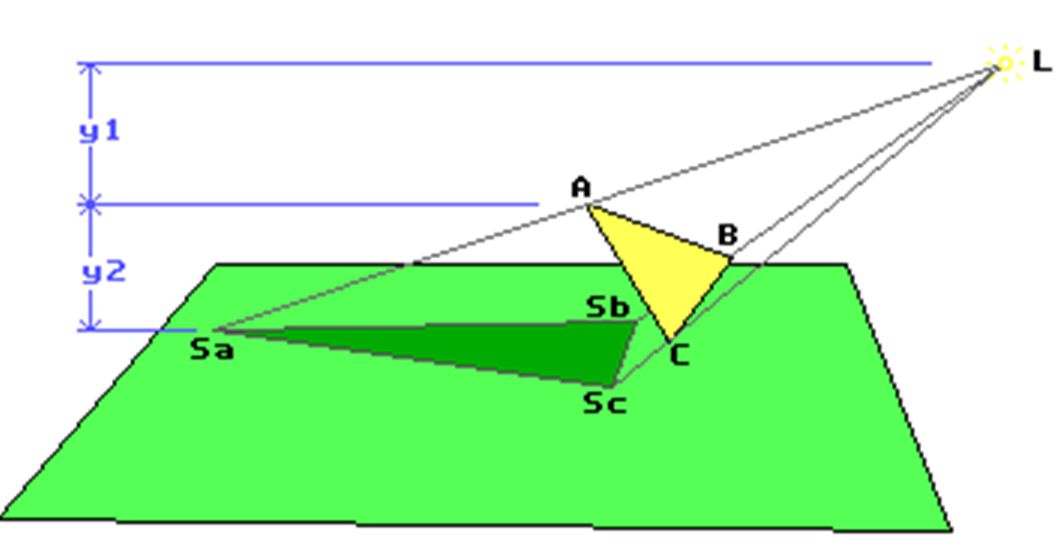
\includegraphics[scale=0.8]{ten}
	 	\centering\caption{Полученная тень от треугольника}
	 \end{figure}
 	\\ Уравнение плоскости выглядит следующим образом:
 	\begin{equation}
 		Q(x, y, z) = Ax + By + Cz + D = 0.
 	\end{equation}
 	\hspace*{5mm} Здесь коэффициенты $A, B, C$ совпадают с координатами нормали к этой плоскости. Координаты нормали плоскости совпадают с координатами нормали треугольника, которые мы посчитали на этапе загрузки сцены.
 	\\ \hspace*{5mm} Для нахождения свободного члена D необходимо подставить координаты любой точки треугольника, например, одной из вершин.
 	\begin{equation}
 		D = -Ax -By -Cz
 	\end{equation}
	\hspace*{5mm}По ходу выполнения программы значение D меняться не будет, поэтому его целесообразно посчитать при инициализации сцены и хранить, как и координаты нормали. Пересчитывать его необходимо только при изменении положения треугольника. 
	\\ \hspace*{5mm} Теперь для нахождения точки пересечения подставим уравнения луча в 
	уравнение плоскости.
	\begin{equation}
		A(x_1 + at) + B(y_1 + bt) + C(z_1 + ct)  + D = 0
	\end{equation}
	Откуда получим
	\begin{equation}
		t = \frac{-(Ax_1 + By_1 + Cz_1 + D)}{(Aa + Bb + Cc)} 
	\end{equation}
	\hspace*{5mm}Если  знаменатель этой дроби равен нулю, значит луч параллелен плоскости, в которой лежит треугольник. Точки пересечения нет.
	\\ \hspace*{5mm} Для нахождения координат точки пересечения надо подставить найденное значение параметра t в уравнения луча. Назовем точку пересечения $D$. Мы получим координаты $x_D, y_D, z_D$.
	\\ \hspace*{5mm} Теперь необходимо определить, попала ли точка D внутрь треугольника. Найдем координаты векторов $AB, BC, CA$ ($A, B, C$ – вершины треугольника) и координаты векторов $AD, BD, CD$. Затем найдем три векторных произведения:
	\begin{equation}
		nA = AB * AD 
	\end{equation}
	\begin{equation}
		nB = BC * BD 
	\end{equation}
	\begin{equation}
		nC = CA * CD
	\end{equation}
	\hspace*{5mm} Эти вектора будут коллинеарные. Если все три вектора сонаправлены, то точка D лежит внутри треугольника. Сонаправленность определяется равенству знаков соответствующих координат всех трех векторов.
	\\ \hspace*{5mm} Операцию проверки принадлежности точки $D$ треугольнику $ABC$ можно ускорить. Если ортогонально спроецировать треугольник $ABC$ и точку $D$ на одну из плоскостей $xOy$, $yOz$ или $xOz$, то попадание проекции точки в проекцию треугольника будет означить попадание самой точки в треугольник (конечно же, если уже известно, что точка $D$ лежит в плоскости, содержащей треугольник $ABC$). При этом число операций заметно сокращается. Так для поиска координат  всех векторов нужно искать по две координаты на каждый вектор, а при поиске векторных произведений нужно искать только одну координату (остальные равны нулю).
	\\ \hspace*{5mm}Для проверки сонаправленности векторов, полученных при вычислении векторного произведения нужно проверить знаки этой единственной координаты для всех трех векторов. Если все знаки больше нуля, или меньше нуля, то вектора сонаправлены. Равенство нулю одного из векторных произведений соответствует случаю, когда точка $D$ попадает на прямую, содержащую одну из сторон треугольника. 
	\\ \hspace*{5mm} Кроме того, перед вычислениями векторов и векторных произведений можно провести простой габаритный тест. Если проекция точки $D$ лежит правее, левее, выше или ниже каждой из проекций вершин треугольника, то она не может лежать внутри.
	\\ \hspace*{5mm} Остается добавить, что для проецирования лучше выбирать ту из плоскостей, площадь проекции треугольника на которую больше. При таком условии исключается случай проецирования треугольника в отрезок (при условии, что проверяемый треугольник не вырожден в отрезок). Кроме того, при увеличении площади проекции уменьшается вероятность ошибки. Для определения такой плоскости проецирования достаточно проверить три координаты нормали треугольника. Если $z$-координата нормали больше (по абсолютному значению) $x$ и $y$, то проецировать надо на плоскость $xOy$. Если $y$ больше чем $x$ и $z$, то проецируем на $xOz$. В оставшемся случае – на $yOz$.
	\subsection{Вывод из конструкторской части}
	\hspace*{5mm} В данном разделе были представлены схемы используемых алгоритмов, а именно алгоритмы z-буфера и холмовой алгоритм. Также было подробно описано таких важных частей как: освещение, просчет теней.	 
%\end{flushleft}
\clearpage
\newpage
\section{Технологическая часть}
%\begin{flushleft}
	\hspace*{5mm} В данном разделе будут рассмотрены требования к программному обеспечению, средства реализации.

	\subsection{Средства реализации}
	\hspace*{5mm} В данной работе используется такие языки программирования как С\# и С++. Изначально был выбран только С\#, но в дальнейшем было решено использовать и С++. Это связано с тем, что этот язык довольно новый для меня и использование его в моем проекте предоставило бы опыт разработки.
	\\ \hspace*{5mm} Весь программный модуль состоит из 2 частей:
	\begin{enumerate}
		\item программа <<Editor>>;
		\item программа <<Viewer>>.
	\end{enumerate}
	\hspace*{5mm} Языком программирования для написания программы <<Editor>> был выбран язык C\#. С помощью C\# можно быстро писать программы под Windows, благодаря удобному синтаксису, интеллектуальным подсказкам и управляемому коду. Используя управляемый код, не нужно заботится о сборке мусора, об указателях и о некоторых базовых структурах и алгоритмах – все это уже реализовано. Главным минусом разработки на C\# является низкая производительность программ. Но это уже компенсируется современным аппаратным обеспечением. Кроме того, в редакторе нам и не требуется высокая производительность, потому что там рассчитываются только карты и нет интерактивных элементов, в отличие от программы просмотра.
	\\ \hspace*{5mm} Языком программирования для написания программы просмотра ландшафтов был выбран язык С++. Язык С++ сочетает в себе удобство с точки зрения структуры кода (объекты, перегрузка функций, операторов, обработка исключений и др.) и программирование на низком уровне (арифметика указателей, ассемблерные вставки, выравнивание памяти, директивы компилятора).Минусы языка С++ тоже имеются: ручная сборка мусора (возможные утечки памяти из-за этого).  
	\\ \hspace*{5mm} В качестве среды разработки была выбрана IDE Visual Studio 2008. Была выбрана именно эта версия, так как она идеально подходит с точки зрения функциональности, простоты использования и используемой памяти по сравнению с более поздними версиями. Также эта среда разработки может сильно оптимизировать код, используя раскрытие циклов, встраивание функций, использование суперскалярных команд процессора SSE и другие, тем самым увеличив производительность.
	\\ \hspace*{5mm} В качестве технологического подхода к разработке проекта был выбран объектно-ориентированный подход. Этот выбор обуславливается легкостью и быстротой разработки программы. 
	\subsection{Структура программы}
	\hspace*{5mm} На рисунке 22 представлена структура разработанного программного продукта.
	\clearpage
	\newpage
	\begin{figure}[h!]
		\centering
		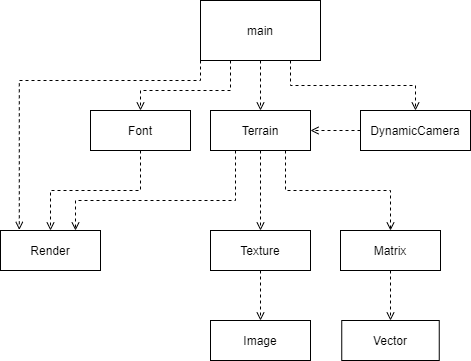
\includegraphics[scale=0.8]{schema}
		\centering\caption{Структура разработанной программы}
	\end{figure}
	\textbf{Main} – модуль, в котором происходит связывание всех компонентов программы.
	\\ \textbf{Tearrain} – описывает непосредственно геометрию ландшафта (вершины, индексы, нормали), текстуры ландшафта, неба, воды.Также этот класс отвечает за визуализацию всех этих объектов. 
	\\ \textbf{DynamicCamera} – реализация камеры, ее передвижения, вращения, а также связь с ландшафтом.
	\\ \textbf{Font} – модуль для инициализации и вывода текста на экран.
	\\ \textbf{Render} – модуль для реализации визуализации в 3-мерном режиме.
	\\ \textbf{Image} – модуль для загрузки и обработки изображений.
	\\ \textbf{Texture} – модуль для загрузки изображений и инициализаций структур.
	\\ \textbf{Vector} – модуль для работы с векторами (сложение, вычитание, скалярное произведение, векторное произведение).
	\\ \textbf{Matrix} – модуль для работы с матрицами (умножение, транспонирование, нахождение обратной). Матрицы используются для реализации композиции трансформаций (перемещение, вращение, поворот), для реализации геометрических алгоритмов.
	\subsection{Входные и выходные данные}
	\hspace*{5mm} \textit{Входными} данными для данной программы является карта высот, карта освещенности и текстура ландшафта, 5 кубических текстур неба и текстура воды в графических файлах в формате “.bmp”, также файл конфигурации, где указаны пути к этим ресурсам. В нем содержится вся информация, необходимая для работы программы. Так же при изображении ландшафта принимаются данные с клавиатуры и мышки, которые интерпретируются как команды пользователя, и в зависимости от них строится последующее изображение.
	\\ \hspace*{5mm}\textit{Выходными} данными программы является анимационный ряд с изображением трехмерного ландшафта, построенного и отображенного на основании входных данных. Также выходными данными является информация о количестве кадров, выводимых на экран за секунду.
	
	\subsection{Интерфейс программы}
	\hspace*{5mm} Ниже представлен интерфейс полученного программного обеспечения. 
	\subsubsection{Интерфейс программы <<Editor>>}
	Интерфейс программы <<Editor>> состоит из нескольких блоков:
	\begin{enumerate}
		\item моделирование;
		\item освещение;
		\item параметры генерации;
		\item предпросмотр
		\item подсчет времени.
	\end{enumerate}
	\hspace*{5mm} В блоке \textit{<<Моделирование>>} пользователю представляется возможность загрузить данные из файла или сгенерировать их самому. Также пользователь может выбрать из ранее подготовленных данных, текстуру неба и воды. Комплекс \textit{<<Освещение>>} можно создать карту освещенности с различно настроенными источниками света в количестве не более 5. Для каждого источника света также можно настривать цвет фонового освещения, диффузного освещения, вектор направления (или позицию с коэффициентами угасания $c_1 c_2 c_3$ для точечных источников). Блок \textit{<<Параметры генерации>>} отвечает за выбор типа ландшафта, размер, материал. \\ \hspace*{5mm} Также пользователю предлагается выбор метода генерации(Холмовой, шум Перлина). Как дополнительными параметрами можно выбрать каким будем итоговая местность: островом или долиной. Также предлагается сгладить ландшафт, а именно сделать его более пологим. Выбрав все выше перечисленные параметры можно воспользоваться отделом \textit{предпросмотр} полученного ландшафта. Как бонус пользователю выводится итоговое время ушедшее для генерации карты высот, освещения и текстуры. На Рисунках 23 и 24 представлен интерфейс модуля <<Editor>>:
	\clearpage
	\newpage
	\begin{figure}[t!]
		\centering
		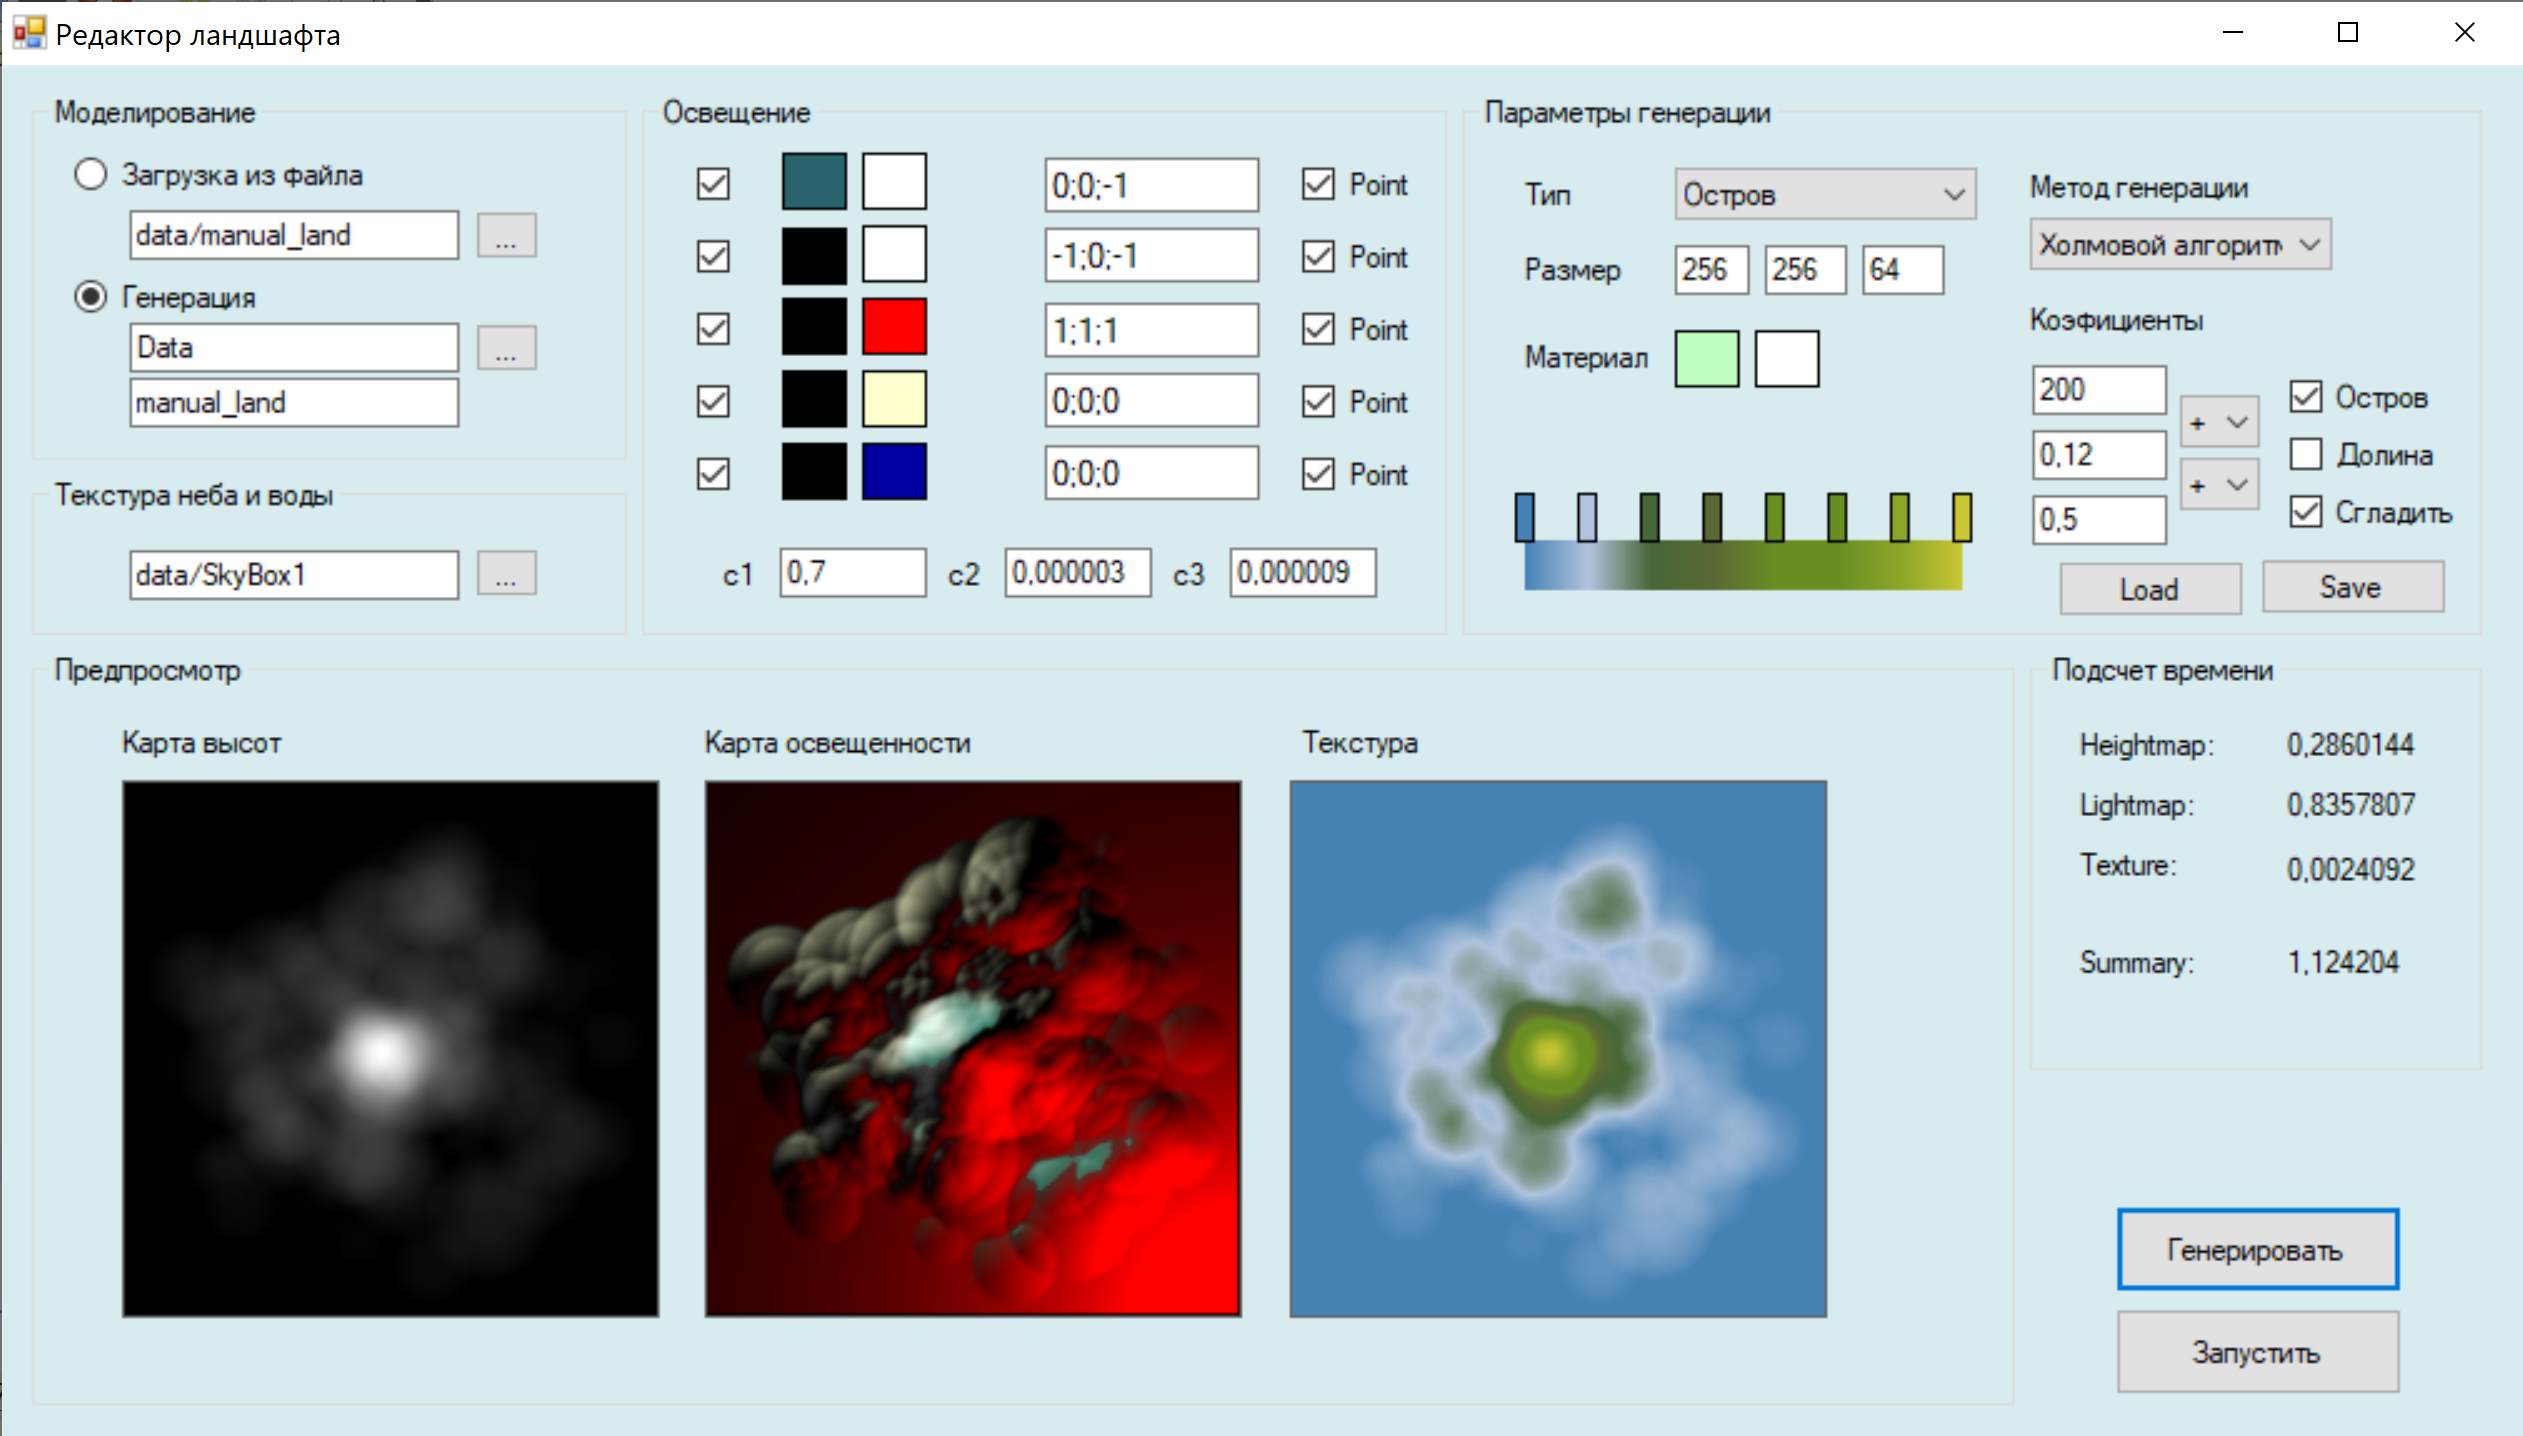
\includegraphics[scale=0.6]{editor1}
		\centering\caption{Интерфейс программы <<Editor>>}
	\end{figure}
	 \begin{figure}[h!]
	 	\centering
	 	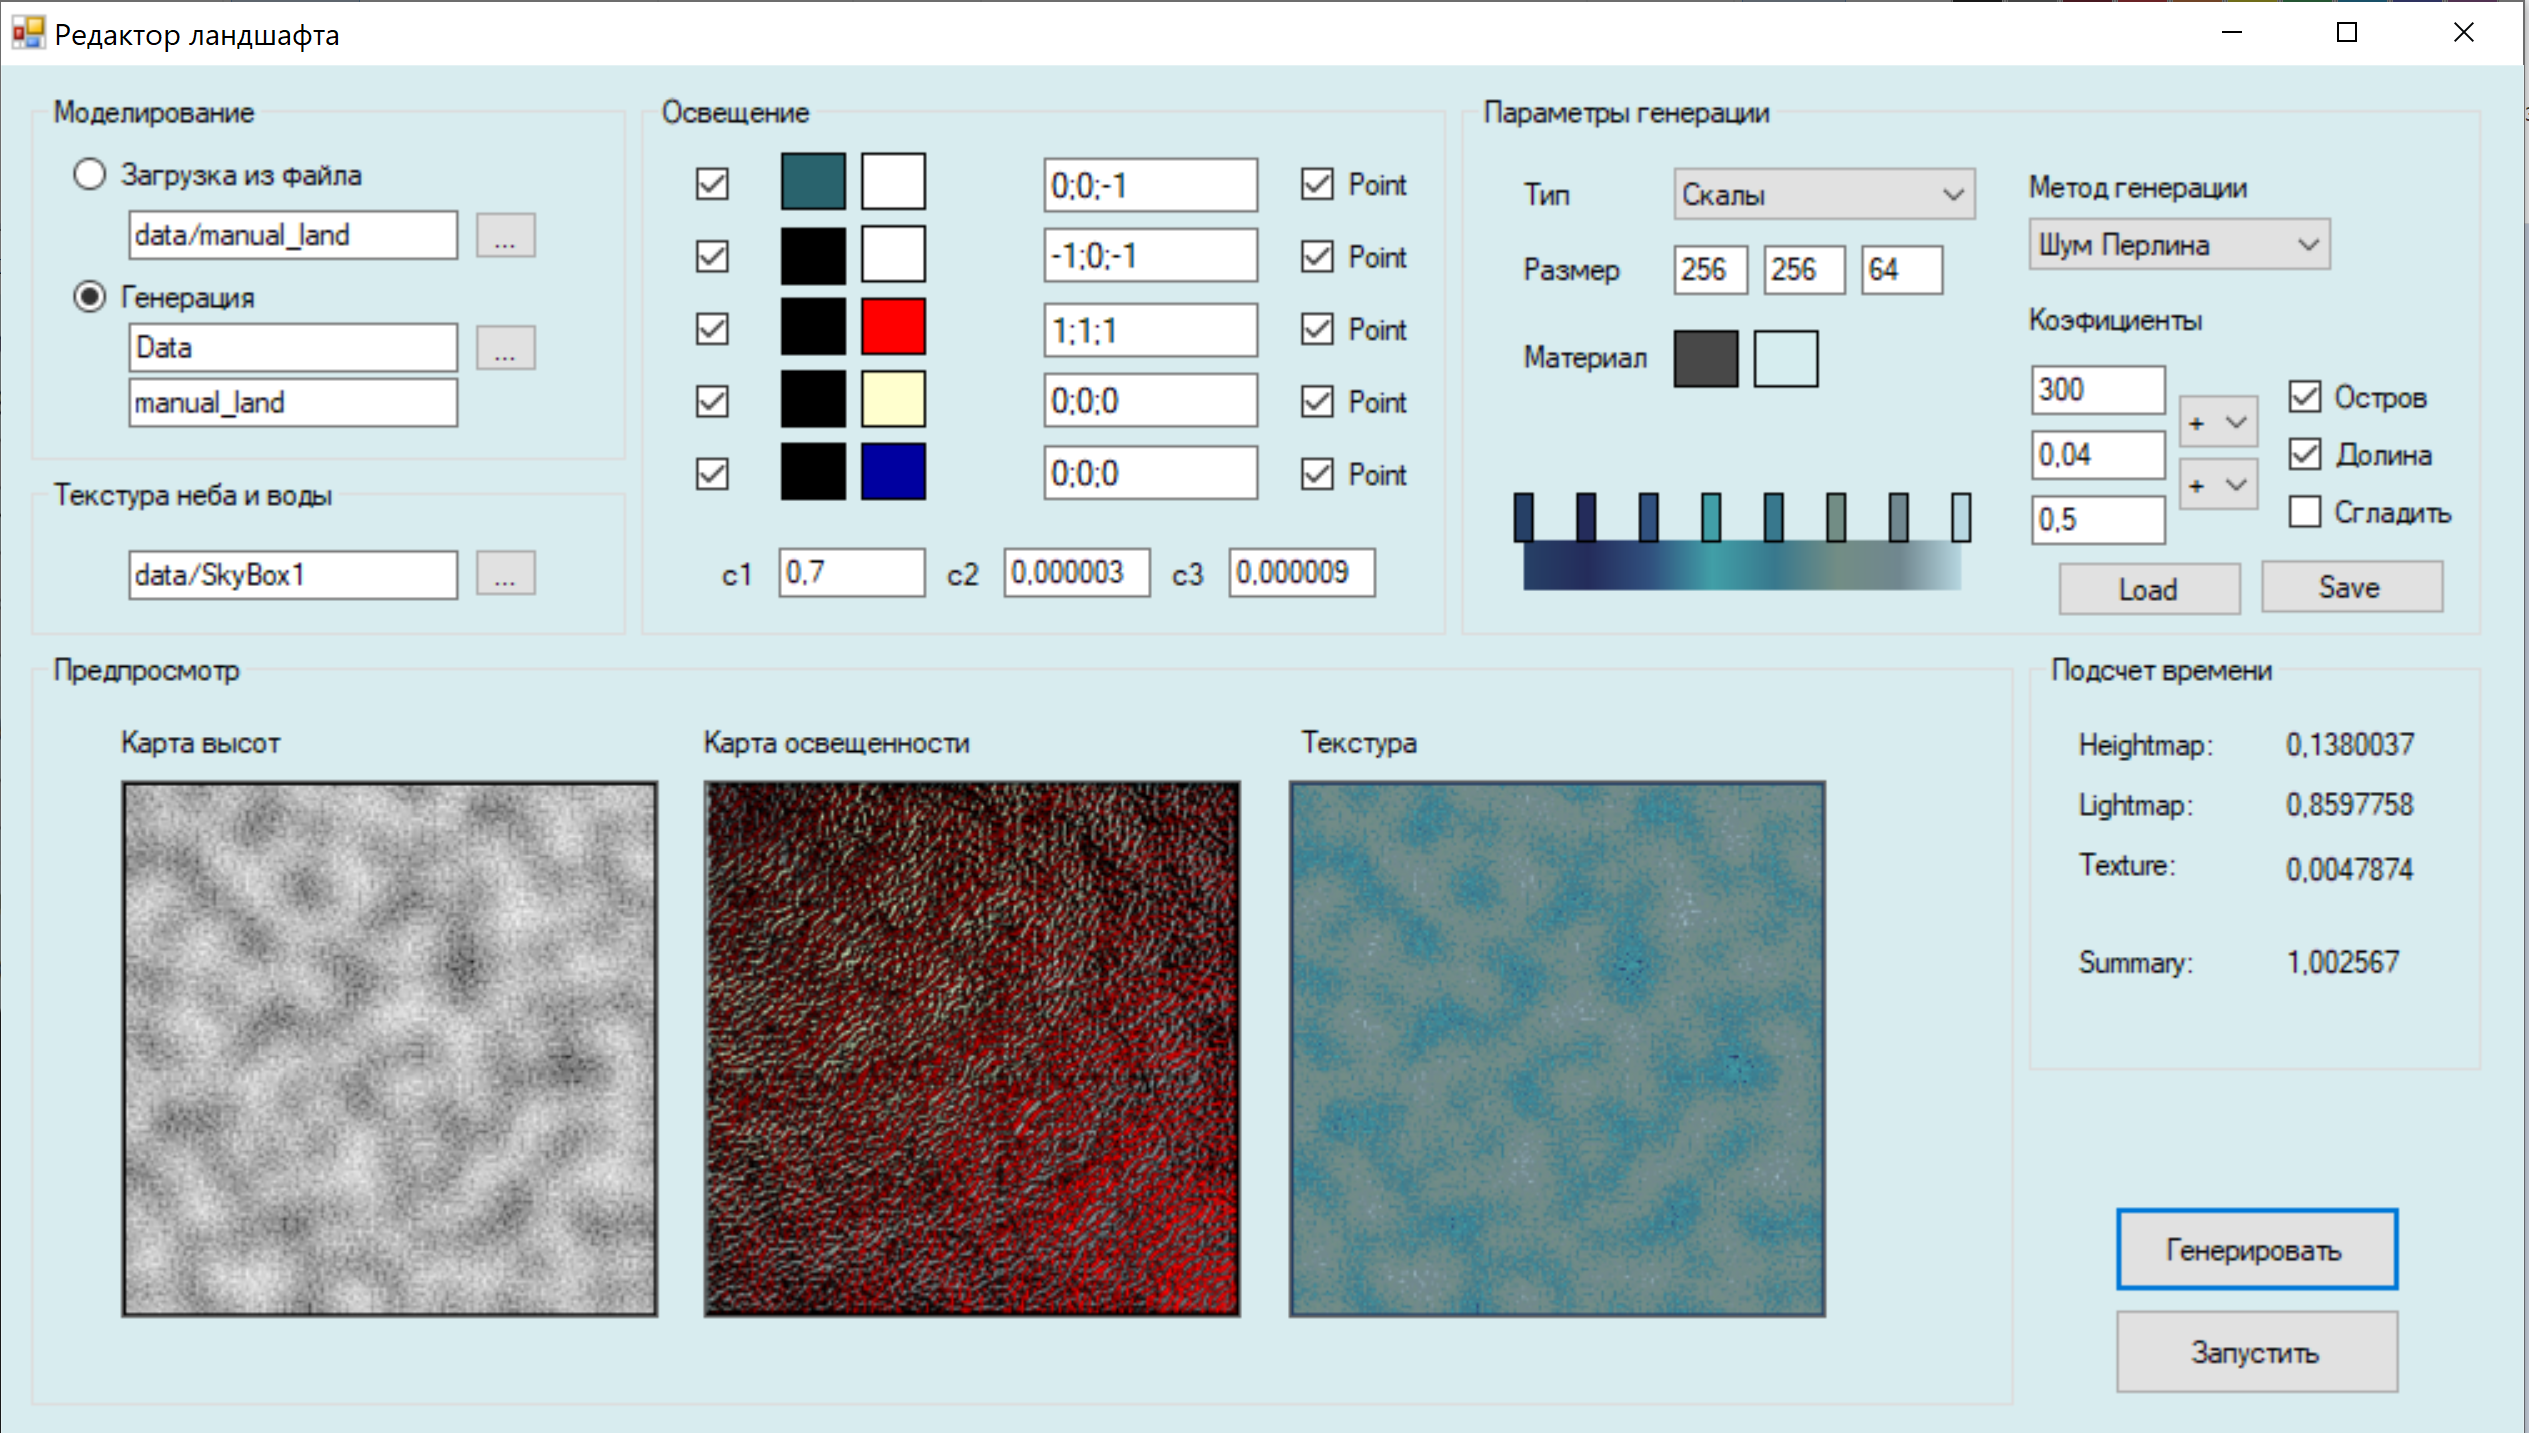
\includegraphics[scale=0.6]{editor2}
	 	\centering\caption{Интерфейс программы <<Editor>>}
	 \end{figure}
 	\subsubsection{Интерфейс программы <<Viewer>>}
 	\hspace*{5mm} Эта программа позволяет просматривать ландшафты в интерактивном режиме, построенные из ранее сгенерированных карты высот, текстур и карт освещенности. Также в этой программе есть поддержка неба, водной поверхности, отражений от воды. 
 	\clearpage
 	\newpage
 	\hspace*{5mm} Интерфейс этой программы довольно простой, что дает возможность любому пользователю разобраться за считанные секунды.
 	\\ W, A, S, D – навигация по пространству
 	\\ $[$ $]$ – увеличение/уменьшение уровня моря. 
 	\\ z, x, c – включение/отключение соответственно текстуры, карты освещенности и карты деталей.
 	\\ v – привязка камеры к поверхности ландшафта (нельзя будет опуститься под поверхность) 
 	На Рисунке 25 представлен интерфейс модуля <<Viewer>>: 
	\begin{figure}[h!]
		\centering
		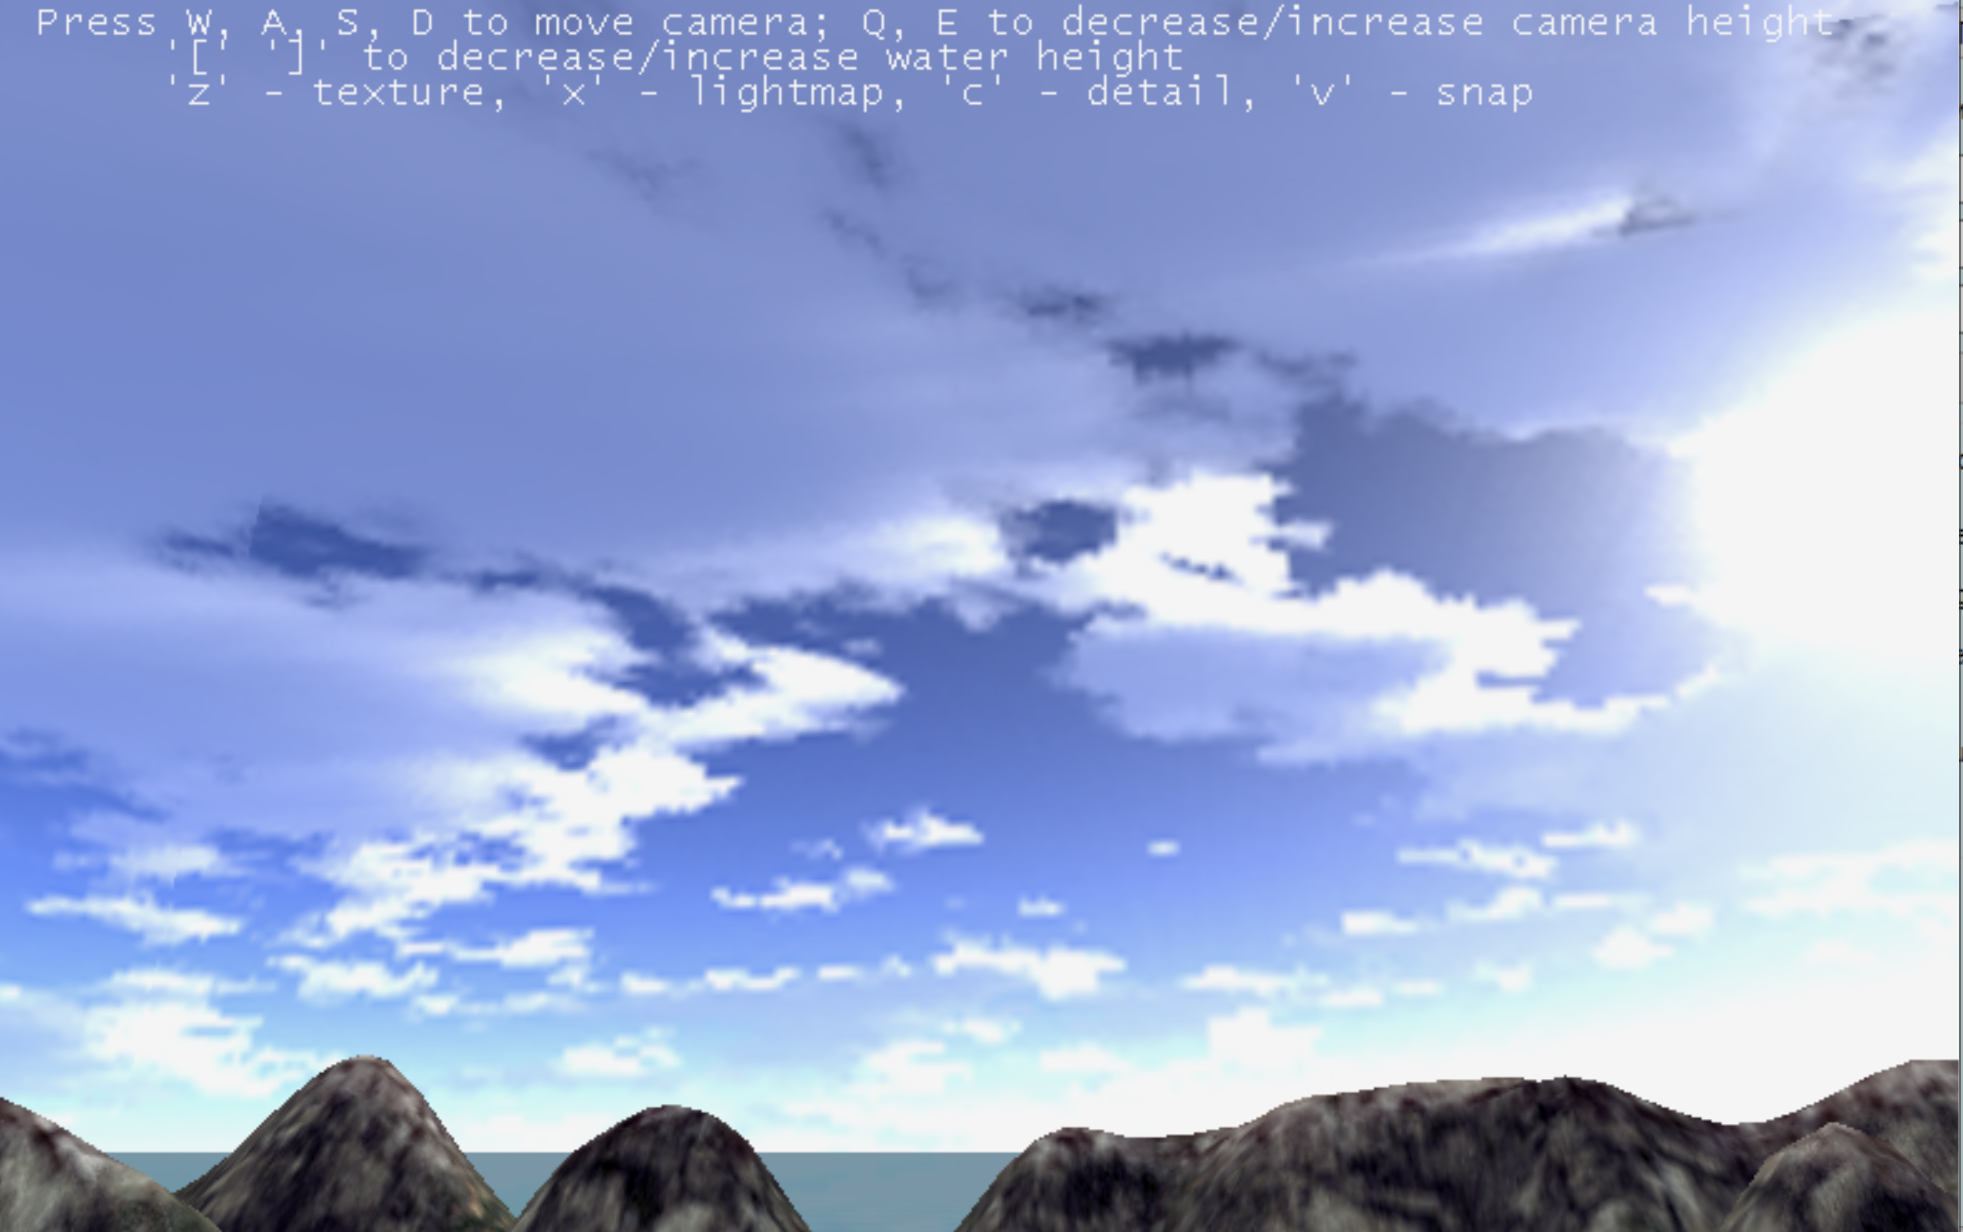
\includegraphics[scale=0.6]{viewer1}
		\centering\caption{Интерфейс программы <<Viewer>>}
	\end{figure}
	\subsection{Вывод из технологической части}
	\hspace*{5mm} В данном разделе было описано и обосновано выбор языка и средств реализации дпнного проекта. Также была предоставлена блок-схема  и описана структура полученного ПО. Был продемонстрировано внутренний интерфейс программы: <<Editor>>, <<Viewer>>.
%\end{flushleft}

\newpage
\section{Исследовательская часть }
%\begin{flushleft}
	\hspace*{5mm} В данном разделе будет проведен эксперимент и сравнительный анализ. Также будут показаны примеры работы программы
	\subsection{Системные характеристики}
	Характеристики компьютера на котором проводился эксперимент:
	\begin{enumerate}
		\item операционная система - Windows 10;
		\item процессор - Intel(R) Core(TM) i7-10510U CPU @1.80GHz 2.30GHz;
		\item объем оперативной памяти - 16 ГБ;
		\item количество ядер - 4;
		\item количество логических процессов - 8;
		\item видеокарта - NVIDIA GeForce GTX 1650 with Max-Q Design;
		\item объем видеокарты - 4 ГБ.
	\end{enumerate}
	\subsection{Постановка эксперимента}
	В рамках данного проекта были проведены эксперименты, описанные ниже:
	\begin{enumerate}
		\item сравнение и анализ времени построения карты освещенности от количества источников света;
		\item сравнение и анализ времени построения карты освещенности от ее размера;
		\item сравнение и анализ числа кадров в секунду, генерируемых программой, от числа граней с наложением карт освещения и без него.
	\end{enumerate}
	
	\subsection{Сравнительный анализ на основе замеров времени работы программы}

	 \hspace*{5mm} На рисунке 26 показаны результаты первого эксперимента, суть которого заключается в анализе времени построения карты освещенности от количества источников света. Количество источниковсвета изменяется от 1 до 5. Для данного эксперимента было выбрано 4 размера карты освещенности: 
	 \begin{enumerate}
		\item 128х128;
		\item 256х256;
		\item 512х512;
		\item 1024x1024.
	\end{enumerate}
	 Ниже приведена полученная диаграмма:
	 \clearpage
	 \newpage
	\begin{figure}[t]
		\centering 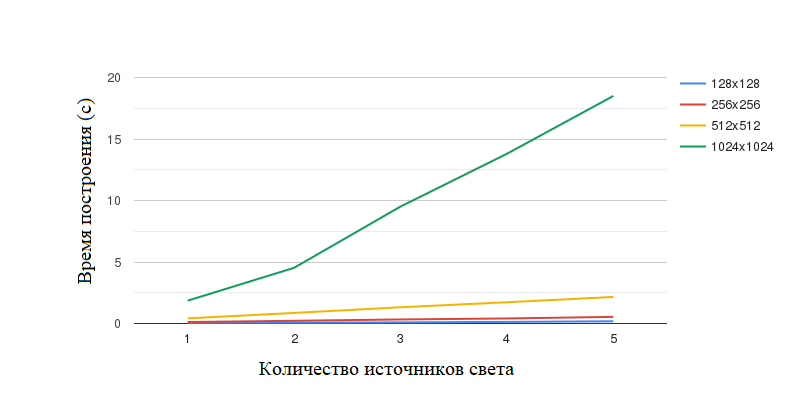
\includegraphics[scale=2]{chart1}
		\centering\caption{Сравнение времени построения карты освещенности от количества источников света.}
	\end{figure}
	\hspace*{5mm} Из данного графика видно, что скорость просчета карты освещенности прямо пропорциональна количеству источников света на сцене. Это соответствует и теоретическим расчетам: каждый пиксель карты освещенности обрабатывается от одного источника  освещения только один раз.
	\\ \hspace*{5mm}  На рисунке 27 показаны результаты второго эксперимента, суть которого заключается в анализе времени построения карты освещенности от ее размера. В данном эксперименте размер карты варьируется в следующих значениях:
	\begin{enumerate}
		\item 128х128;
		\item 256х256;
		\item 512х512;
		\item 1024x1024;
		\item 2048x2048.
	\end{enumerate}
	Ниже приведена полученная диаграмма:
	\clearpage
	\newpage 
	\begin{figure}[h]
		\centering 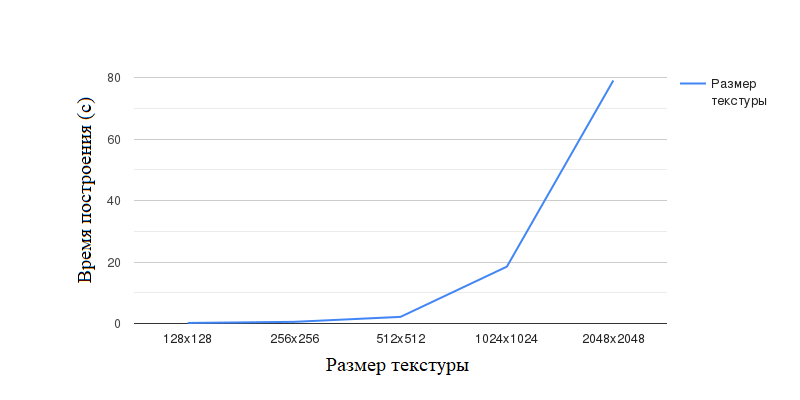
\includegraphics[scale=2]{chart2}
		\centering\caption{Сравнение времени построения карты освещенности от ее размера.}
	\end{figure}
	 Из данной зависимости становится понятным, что затрачиваемое время на просчет карты освещенности  $~2^N$, где $N$ – размер карты.
	\\ \hspace*{5mm} Третий эксперимент был проведен, для того чтобы сделать анализ зависимости числа кадров в секунду, генерируемых программой, от числа граней с наложением карт освещения и без него, для двух способов наложения карт освещения – двухпроходного рисования и мультитекстурирования. На Рисунках 28 и 29 показаны двухпроходное рисование и мультитекстурирование соответственно:
	\begin{figure}[h]
		\centering 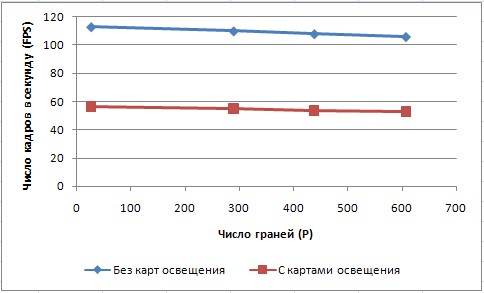
\includegraphics[scale=1]{chart3}
		\centering\caption{Двухпроходное рисование.}
	\end{figure}
	\clearpage
	\newpage
	\begin{figure}[h]
		\centering 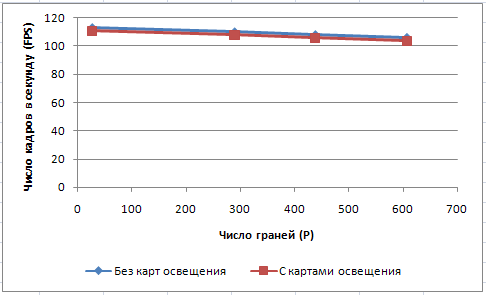
\includegraphics[scale=1]{chart4}
		\centering\caption{Мультитекстурирование.}
	\end{figure}
	\hspace*{5mm} Суть \textit{двухпроходного рисования} в том, что каждая грань рисуется два раза – один раз с основной текстурой, второй раз с картой освещения в режиме «смешивания» - поэтому скорость рисования сцены падает в два раза. \textit{Мультитекстурирование} – операция, реализованная аппаратно и позволяющая наложить несколько текстур в один проход, поэтому скорость рисования сцены падает очень незначительно. В обоих случаях число кадров в секунду выше требуемого для интерактивных программ уровня в 25 кадров/с.
	\\ \hspace*{5mm}На Рисунке 30 показано сравнение использования карт освещения с простой моделью освещения, реализованной программно (освещенность вычисляется для каждой грани в момент рисования):
	\begin{figure}[h]
		\centering 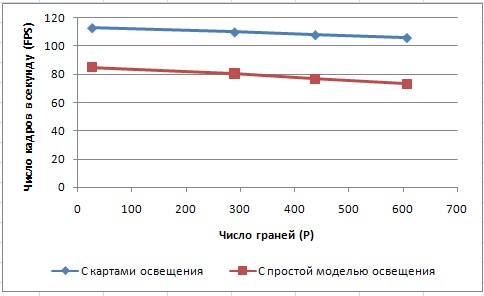
\includegraphics[scale=1]{chart5}
		\centering\caption{Сравнение использования карт освещения с простой моделью освещения.}
	\end{figure}
	\\ \hspace*{5mm} Как видно из Рисунка 30, использование карт освещения опережает по скорости даже простую модель освещения, позволяя при этом получить гораздо более реалистичное изображение.
	\subsection{Примеры работы программы}
	\hspace*{5mm} Ниже на Рисунках 31 и 32 показаны примеры работы программы:
	\begin{figure}[h]
		\centering 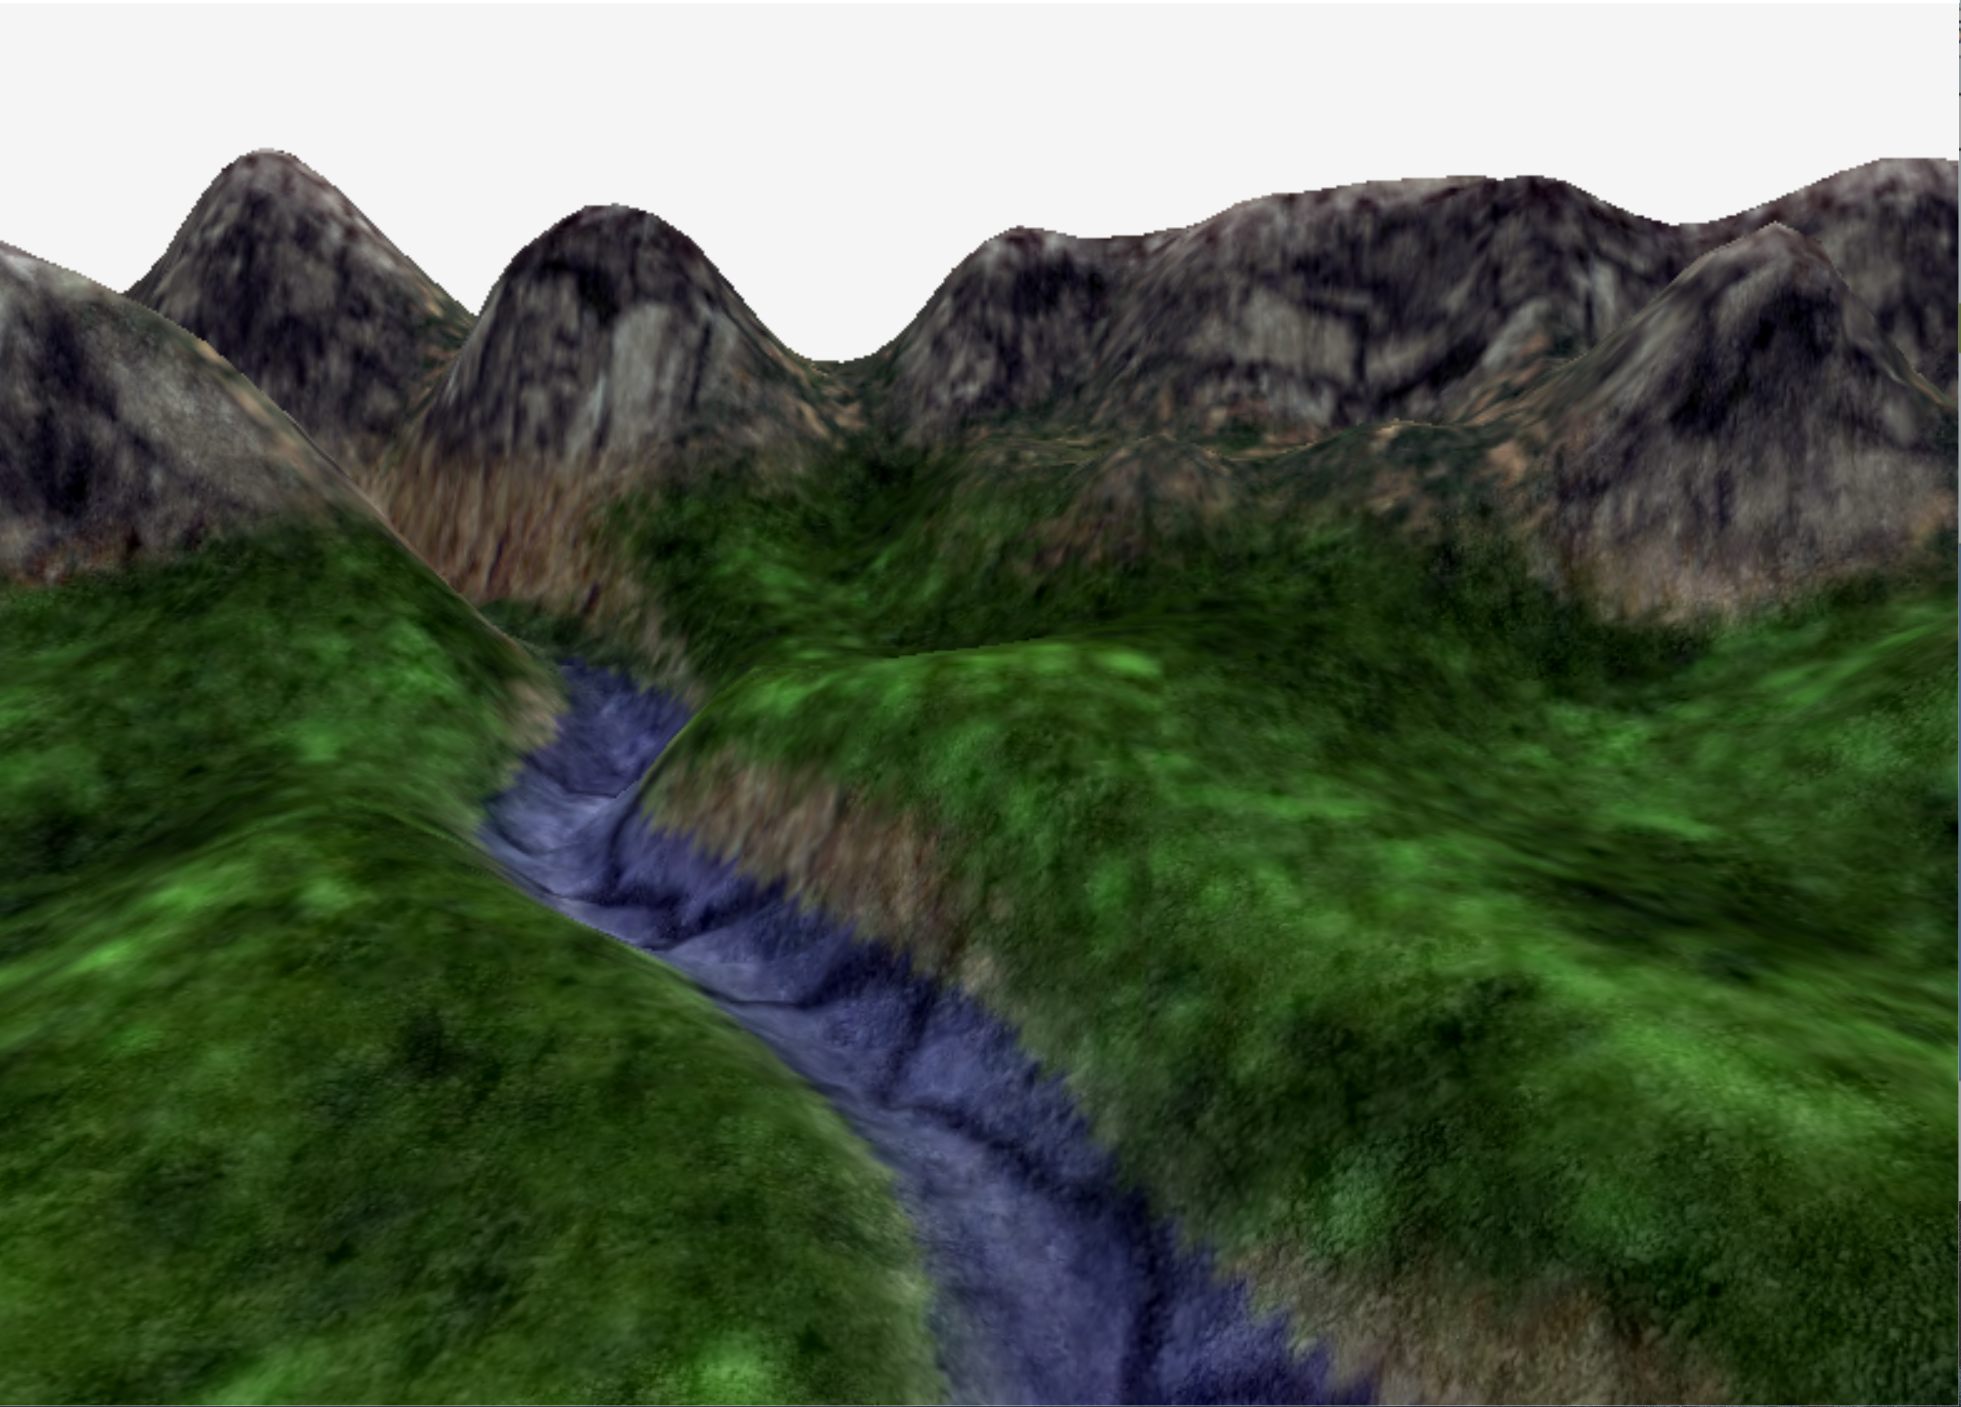
\includegraphics[scale=0.6]{primer1}
		\centering\caption{Пример работы программы без текстуры неба.}
	\end{figure}
	\begin{figure}[h!]
		\centering 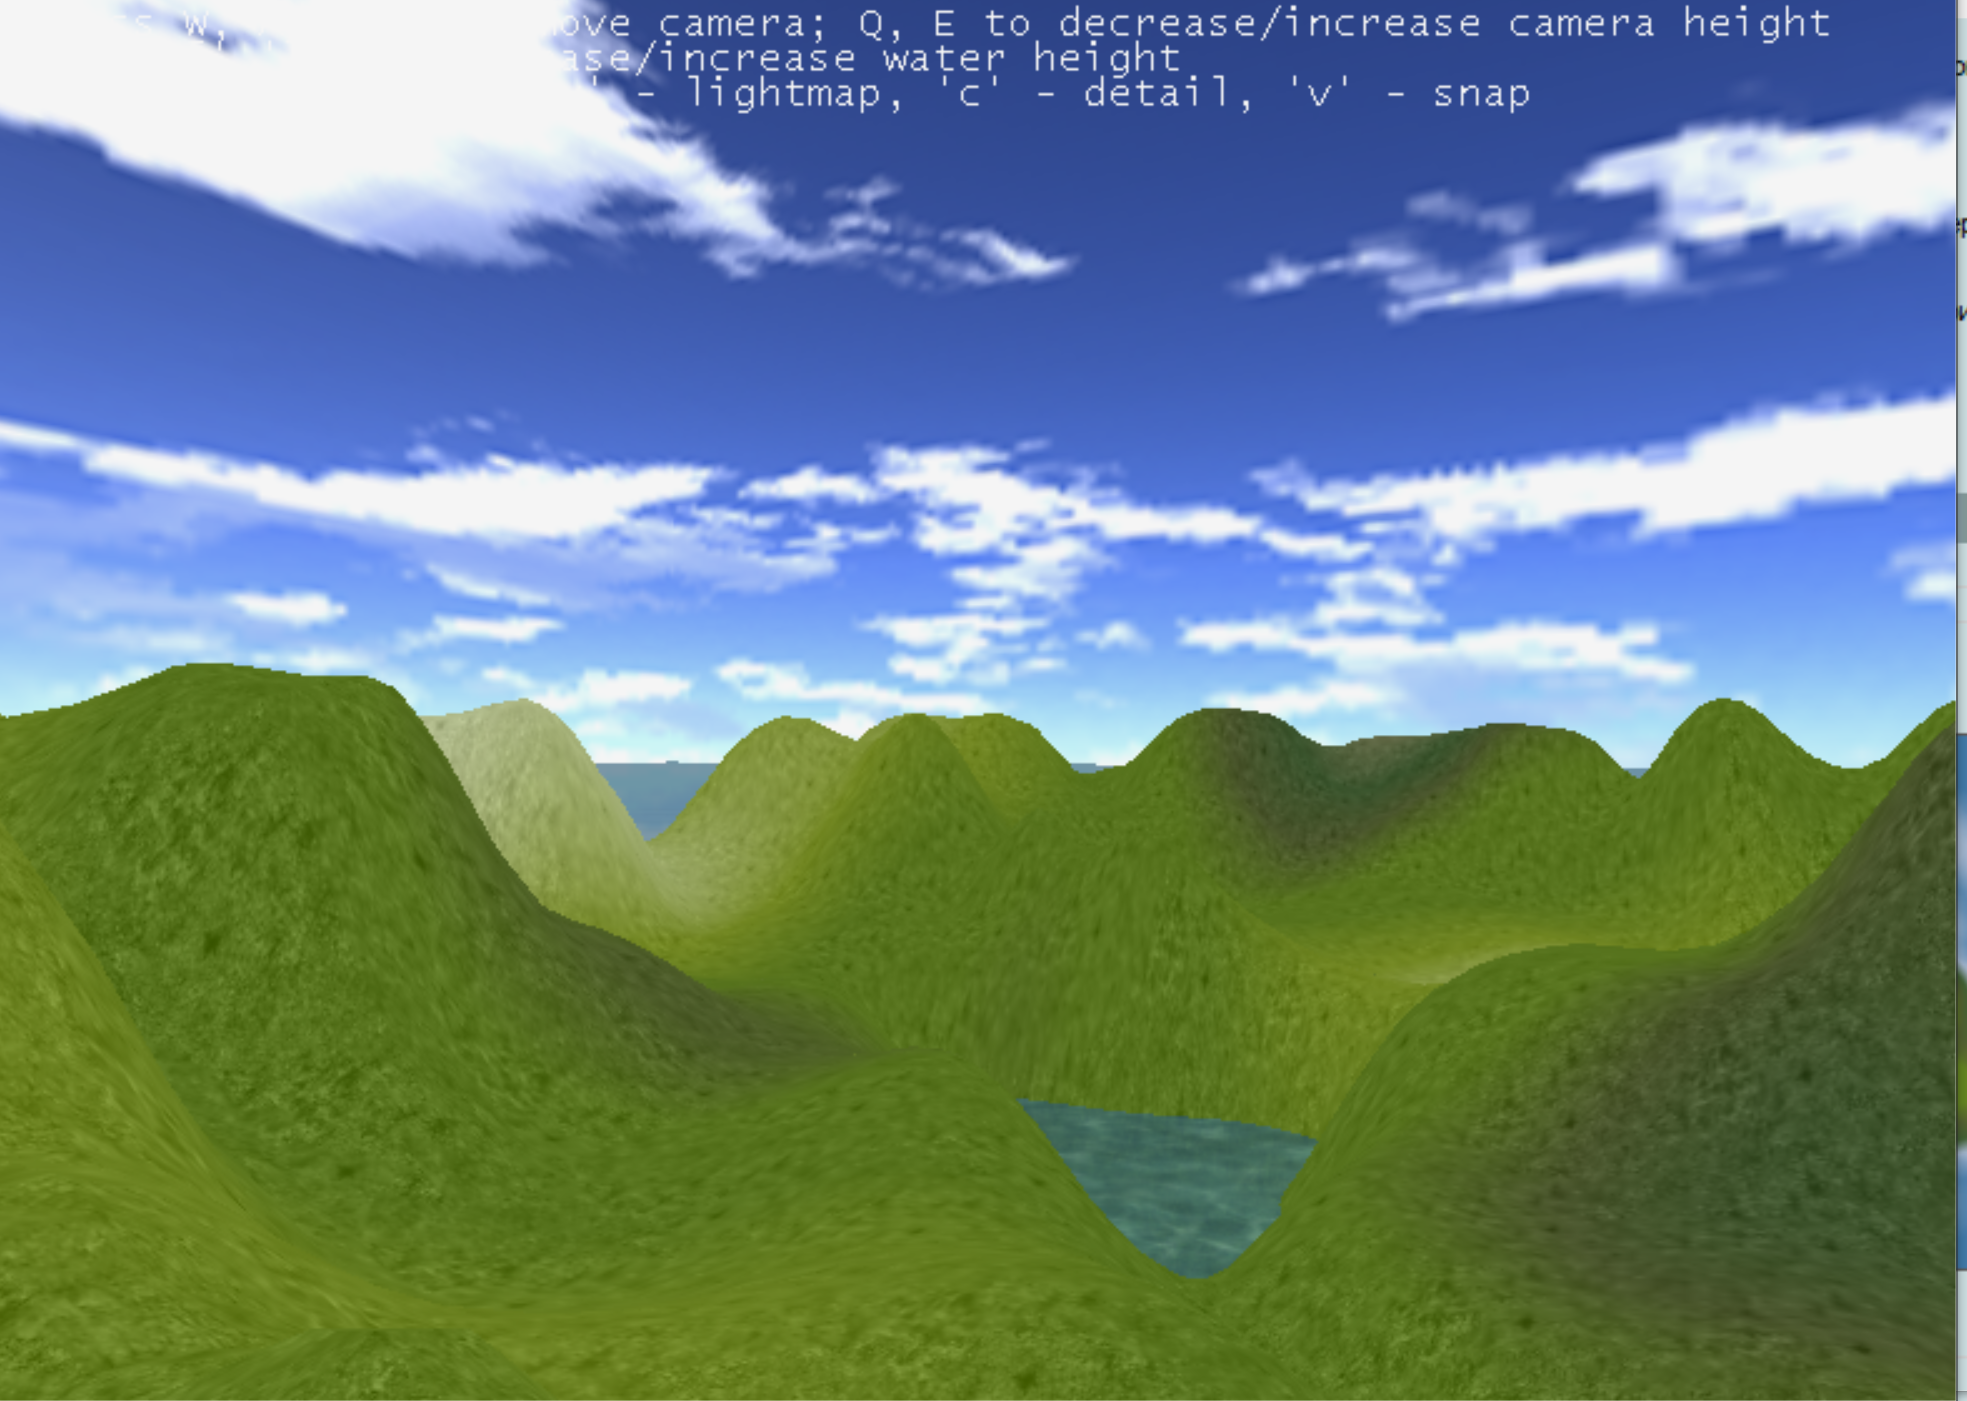
\includegraphics[scale=0.6]{primer2}
		\centering\caption{Пример работы программы с текстурами воды и неба.}
	\end{figure}
	\clearpage
	\newpage
	\subsection{Вывод из исследовательской части}
	\hspace*{5mm} В данном разделе были показаны примеры работ программы. Также были продемонстрированы результаты исследования зависимости времени создания карты освещенности от количества источников света. Это исследование показало нам, что скорость просчета карты освещенности прямо пропорциональна количеству источников света на сцене. Это соответствует и теоретическим расчетам: каждый пиксель карты освещенности обрабатывается от одного источника  освещения только один раз. Из вторго эксперимента становится понятным, что затрачиваемое время на просчет карты освещенности  $~2^N$, где $N$ – размер карты.
	\clearpage
%\end{flushleft}

%\begin{flushleft}
	\section*{Заключение}
	\addcontentsline{toc}{section}{Заключение}
	\hspace*{5mm}Разработанный программный комплекс обеспечивает возможность генерации или загрузки карт высот, карты освещенности и текстуры. Также он позволяет строить изображения ландшафта с наложением текстуры в реальном времени. Проведены исследования работы алгоритмов на различных наборах исходных данных. 
	\\ \hspace*{5mm}Результаты работы программы можно использовать для рисования освещенной сцены в реальном времени, с такой высокой скоростью, которая невозможна без использования предварительного расчета освещения. Получаемые изображения обладают высокой степенью реалистичности.
	Благодаря тому, что форматы результатов (набор карт освещения) являются широко  распространенными в современных приложениях трехмерной графики, программу можно легко использовать на практике для решения реальных задач.
	\\ \hspace*{5mm}Тем не менее, существует множество путей усовершенствования описанного программного комплекса:
	\begin{enumerate}
		\item генерируемые текстуры ландшафта все-таки выглядят не очень реалистично, из-за того, что на них не накладывается текстура грунта, травы;
		\item в данной программе нет генерируемых растительности и деревьев, а также смена времени суток.
		Внесение данных нововведений, несомненно, добавило бы реалистичности в генерируемый мир и расширило бы его возможности.
	\end{enumerate} 
	   
%\end{flushleft}

\clearpage
\newpage

\printbibliography
\addcontentsline{toc}{section}{Список литературы}

\end{document}